\documentclass{article}[11pt]
\usepackage[ascii]{inputenc}
\usepackage[T1]{fontenc}
\usepackage{geometry}
\geometry{verbose,letterpaper,lmargin=1in,rmargin=1in,tmargin=1in,bmargin=1in}

\usepackage{fancyhdr}
\pagestyle{fancy}
\setlength{\headheight}{24pt}
\usepackage{amsmath}
\usepackage{amssymb}
\usepackage[numbers,sort&compress]{natbib}
\usepackage[compact]{titlesec}
\usepackage{floatflt}
\usepackage{longtable}
\usepackage{wrapfig}
\usepackage{floatrow}
\usepackage{graphicx}
\usepackage{tabularx}
\usepackage{subcaption}
\usepackage{url}
\usepackage{color}
\usepackage{pdfpages}


\usepackage{mathptmx}
\usepackage[english]{babel}
\usepackage{amsmath}
\usepackage{amssymb,amsfonts,textcomp}
\usepackage{array}
\usepackage{supertabular}
\usepackage{multirow}
\usepackage{hhline}
\usepackage{enumitem}
\usepackage{xspace}
\usepackage{upgreek}
\usepackage{microtype}
\usepackage{lineno}
%\linenumbers
\usepackage{stackrel}
\usepackage{accents}
% Markus
\usepackage{verbatim}
% Riccardo
\usepackage{todonotes}

% hyperref likes to be last
\usepackage[colorlinks, urlcolor=blue, linkcolor=blue]{hyperref}
\makeatletter
\newcommand\arraybslash{\let\\\@arraycr}
\makeatother
\setlength\tabcolsep{1mm}

\setlength{\parindent}{0cm}
\setlength{\parskip}{1.0ex plus 0.5ex minus 0.2ex}
%
% Macros for this paper go here.
%
\renewcommand\arraystretch{1.3}
\newcommand{\cpp}{C\kern-0.15ex{+}\kern-0.1ex{+}\xspace}
\newcommand{\art}{\textit{art}\xspace}
\newcommand{\pythia}{\textsc{Pythia8}\xspace}
\newcommand{\nova}{NOvA\xspace}

%%% Macros for comments in the proposal (can be deleted later)
\newcommand{\jim}[1]{[{\sc Jim:} {\color{green}\textit{#1}}]}


\begin{document}

%\section{PROJECT SUMMARY / ABSTRACT}
%\input{project_summary}

%\section{DOE COVER PAGE}
% Tell TeXShop about the master file
% !TEX root = ExaTrkX_proposal.tex
%
%
% DOE COVER PAGE
% (PART OF PROJECT NARRATIVE)
%
% The following proposal cover page information may be placed on a plain
% page. No form is required. This cover page will not count in the
% project narrative page limitation.
%

% https://en.wikibooks.org/wiki/LaTeX/Title_Creation

\begin{center}
\thispagestyle{empty}
%\section*{} 
\vspace{10pt}
\setlength{\parskip}{1em}

{ \Large {\bf   ATLAS HL-LHC Computing Conceptual Design Report}}

%Editors: Paolo Calafiura (LBNL) and Davide Costanzo (University of Sheffield)\\

%\hspace{1cm}

%{\bf Contributors:} 

%Visualistion section: R.M. Bianchi <riccardo.maria.bianchi@cern.ch>, S.Chekanov <chekanov@anl.gov>  (to be added)


\vspace{15em}
\missingfigure[figwidth=7cm]{Image: a busy HL-LHC event, showing a large number of tracks/vertexes (Riccardo)}



 
\end{center}
\newpage

\tableofcontents
\newpage

\setcounter{page}{1}


\section{Introduction}
%Davide+Paolo
  ATLAS HL-LHC precision physics program will require more statistics, but also increased accuracy in the simulation and reconstruction of ATLAS physics objects. Preliminary ATLAS projections of computing resources (CPU and storage) show significant deficits starting at the beginning of Run 4 (Figure~\ref{fig:2018Res}). If not addressed, these deficits would likely limit ATLAS physics reach.
  
 The goals of this ATLAS Conceptual Design Report (CDR) for HL-LHC Computing are to:
\begin{enumerate}
    \item Establish a baseline computing model, data rates, computing and storage projections for Run 4 and Run 5, including the evolving roles of the Computing Centers,
    \item Establish anticipated cost drivers and infrastructure assumptions,
    \item Outline technological risks and major areas of R\&D.
\end{enumerate}

\begin{figure}[htb!]
  \centering
  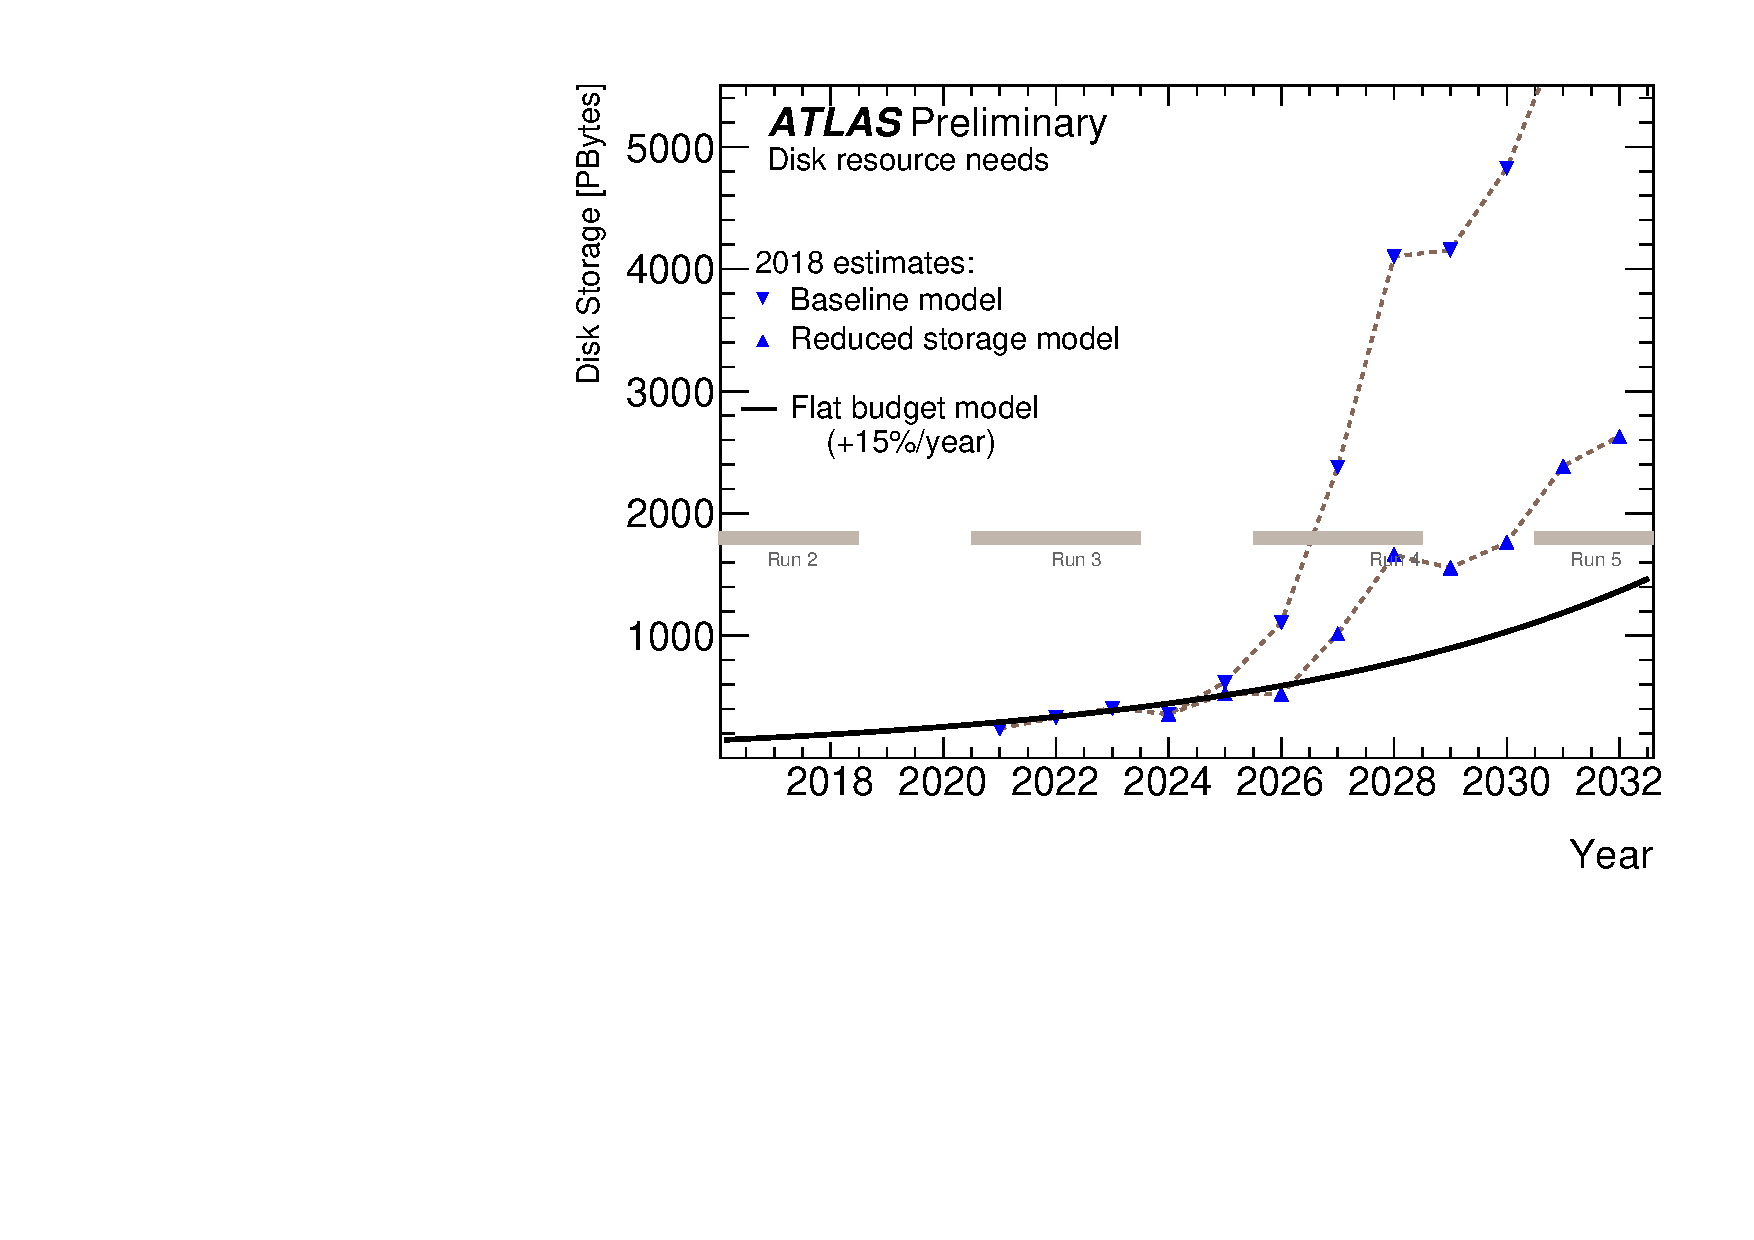
\includegraphics[width=0.48\textwidth]{figures/diskHLLHC_2018.pdf}
  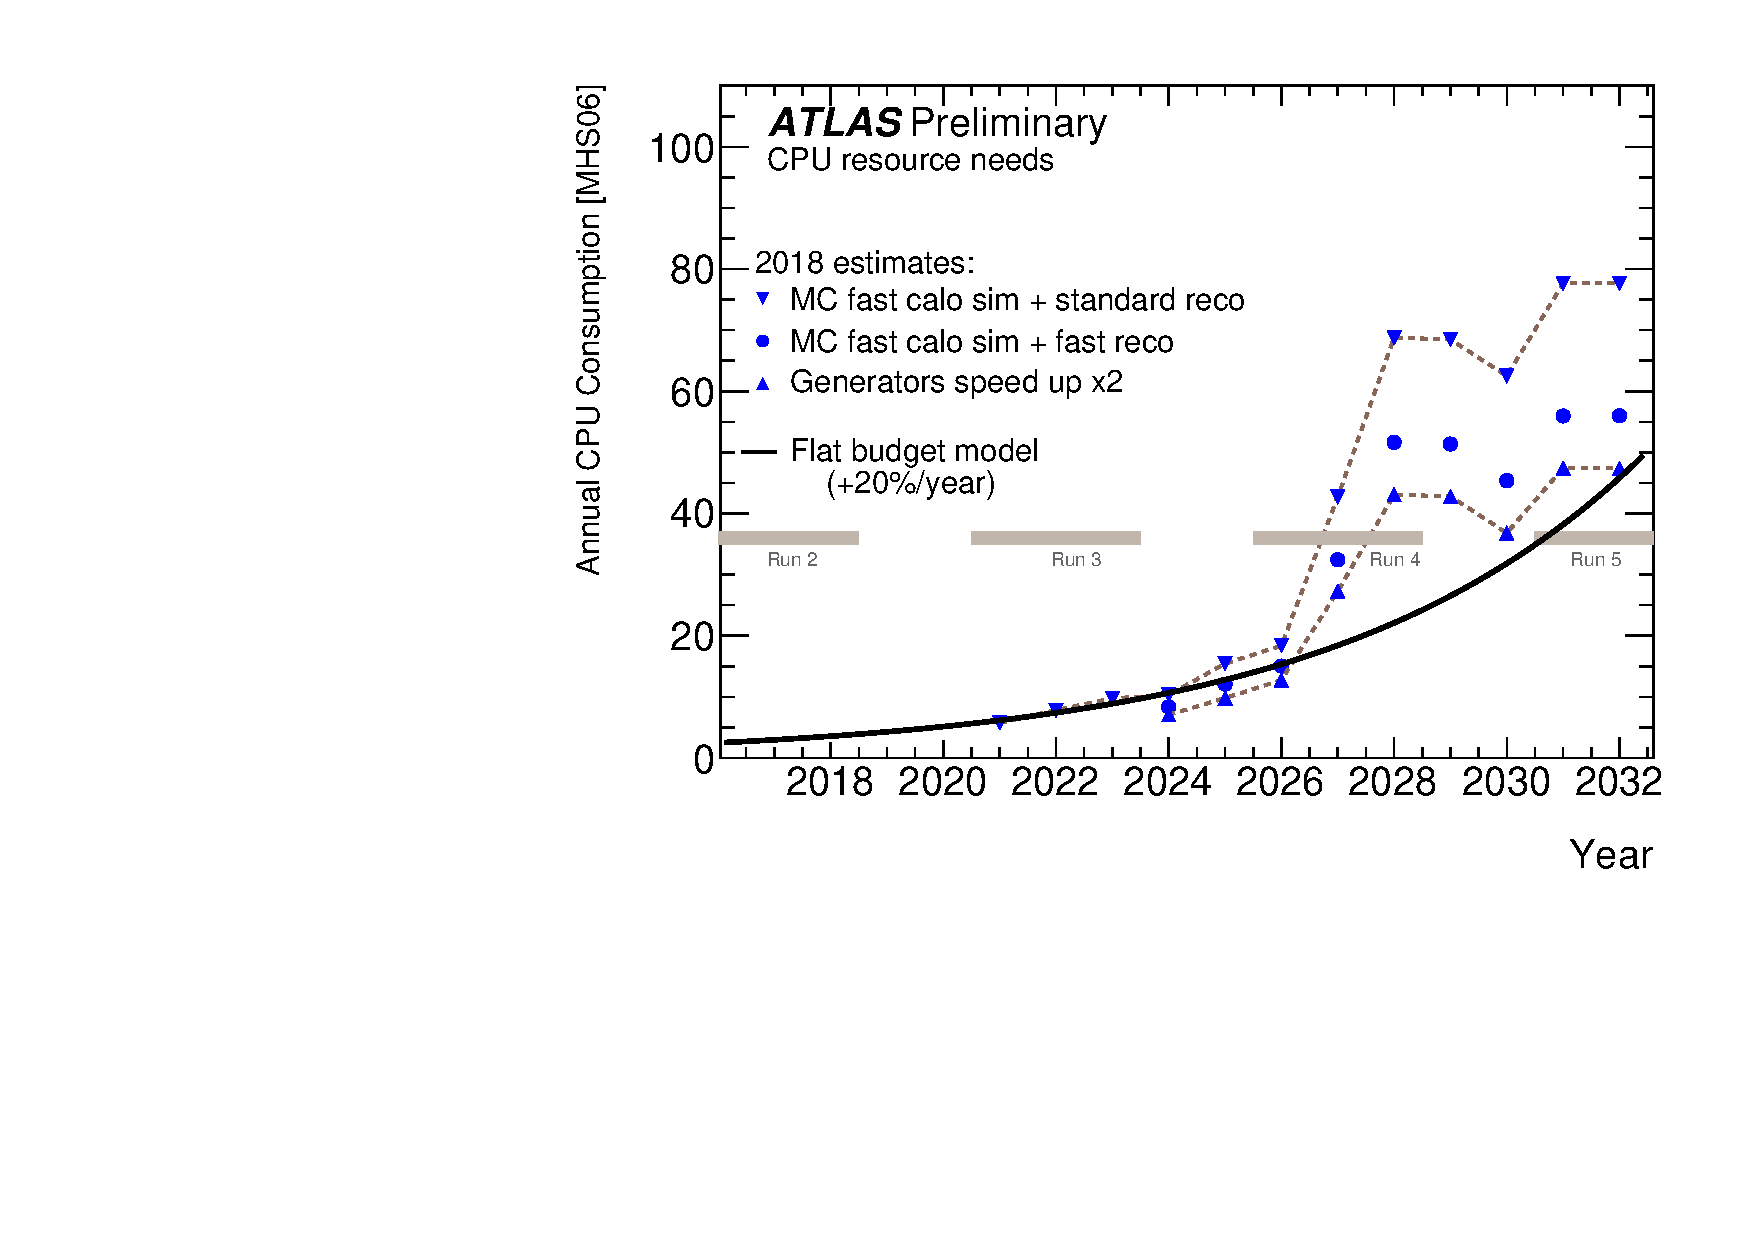
\includegraphics[width=0.50\textwidth]{figures/cpuHLLHC_2018.pdf}
  \caption{ 
Estimated total resources needed for the years 2018 to 2032 for both data and simulation processing {\bf Left:} Disk (in PBytes)  {\bf Right:} CPU (in MHS06).}
  \label{fig:2018Res}
\end{figure}


The CDR process started in the Fall 2019 by reaching out to the ATLAS Computing, Software, and Upgrade Physics communities. This document reflects their input on R \& D priorities and ideas, and on the expected impact of projected storage and computing resource shortages on the HL-LHC Physics program.  It is organized along the traditional ATLAS Computing and Software domains (e.g. core software, simulation, distributed computing, analysis, etc.). 

The document attempts to evaluate the impact on resources and physics reach of the experiment under three scenarios:
\begin{description}
  \item[Conservative] HL-LHC Computing Model and Software are an incremental evolution of the Run 3 one. This would include e.g. 30\% storage savings deriving from the Run 3 Analysis Model \cite{ref:AMSG3}.
  \item[Baseline] Assume success of well-established R\&D projects, e.g. using FastCaloSim \cite{ref:FastChain} for 75\% of MC simulated events, or direct-from-tape processing\cite{ref:DataCarousel}.
  \item[Aggressive] Assume success of one or more "paradigm-shift" R\&D initiatives, such as accurate, fast detector simulation\cite{ref:CaloGAN} that we use to produce 90\% of our simulated events.
\end{description}
 It provides updated estimates of ATLAS computing resource needs under the three scenarios. 

At the end, it describes an initial set of goals and high-level milestones for the ATLAS HL-LHC Computing and Software R\&D program.

\section{Overview}
\label{sec:overview}
The objective of the computing and software project in ATLAS is to enable the Collaboration to fully exploit the HL-LHC dataset, whilst limiting the costs associated with computing. This Conceptual Design Report (CDR) summarises the current approaches being taken and plans being laid within ATLAS to meet this challenge. In particular areas where greater investment will be required in the coming years are highlighted. Based on the present Computing Model, an extrapolation of the resources requirements needed for HL-LHC indicates a significant shortfall in disk and compute power. This is true even if the investment from funding agencies continues to increase at the rate established in  previous years. A significant investment in person power to carry out the necessary research and development to address this shortfall and thereby avoid excessive computing costs in the future. The long term sustainability of the ATLAS software therefore depends on engaging individuals whose expertise and specialism is software development. Given the complexity of the ATLAS detector and software project, sustainability over the next two decades will require that senior decision makers and funding agencies are willing to invest in people, and award personal research grants to those who whose specialism in in software and computing development. A more modern and open software architecture will help attract early career researchers with a software background, but sustainability requires that such individuals have a realistic prospect of long term employment in the field. \\
 
To sustain HL-LHC data analysis, Monte Carlo events will need to be generated and simulated in prodigious numbers - it is likely that approximately ten times more MC statistics will be required during Run 4, which implies at least 200 billion events. \\

Event generation for ATLAS has been a large consumer of compute resources to date (approximately 10-15\%) and it is likely to become more prominent in Run 4, as many measurements and searches will require higher precision, which implies use of NLO or NNLO generators. As well as software development to maximise efficiency and perhaps make use of accelerators, careful optimisations of physics choices, bias the event generation as a function of a kinematic quantity of interest (thereby reducing the number of events needed), suppressing negative event weights, and even sharing generated events between collaborations, will all contribute to ensuring that event generation is sustainable in Run 4. It should be noted that event generators are typically developed by small teams of theorists, whose primary concerns are not related to computing. Endeavours to increase collaboration on software across the field, especially the High Energy Physics Software Foundation (HSF), are of crucial importance if applications such as event generation are to be scaled up to HL-LHC demands. \\ 

ATLAS currently expends most (60\%) of its CPU resources on detector simulation. Approximately half of the events are produced with so-called full simulation, using the Geant4 physics library, with the rest coming from fast simulation which uses a parameterised model of the calorimeter response. Full simulation uses around eight times more compute resources than fast. ATLAS aims to raise the level of fast simulation to 75\% at the very least during Run 4. However, ATLAS will need to extend the fast simulation concept to all parts of the detector, including the inner tracker as well as the calorimeter. Novel simulation techniques made possible by deep learning may also prove highly effective at speeding up aspects of the simulation. Use of full simulation will remain unavoidable for certain applications, and for this reason ATLAS will collaborate closely with the Geant4 team to ensure the best possible physics fidelity for the lowest possible expenditure of resources. Finally, ATLAS must ensure that the compute costs of trigger simulation remain under control, especially as hardware based tracking will be used in the HL-LHC trigger system. \\

The reconstruction stage, which is fully under the responsibility of ATLAS, will benefit enormously from the Phase II upgrade to the inner tracker, the ITk. As well as providing exceptional physics performance, it is also optimised to minimise CPU consumption of tracking despite the much higher pile-up at the HL-LHC. At the same time, ATLAS is pursuing several promising avenues of software optimisation, which together with the ITk should ensure sustainable reconstruction in Run 4. These developments include improvements and optimisations to the classical algorithms that can further exploit the ITk design and provide very substantial CPU savings with tolerable loss of physics performance. ATLAS is also implementing a new cross experiment tracking software, which benefits from a modern design with a light-weight event data model. This is expected to yield further savings and efficiencies. (write something here quantitative). Novel approaches based on machine learning, or new non-ML algorithms, may be able to improve the physics and computing performance further. Finally, ATLAS is investigating the possibility of allowing accelerators to be used for aspects of the reconstruction, as part of the heterogeneous software programme. All of these improvements require a determined investment to maintain and increase the available person power. \\

ATLAS is implementing a new analysis model which aims to reduce the disk footprint occupied by analysis formats. It is based around two formats, one with a size of at most 50KB/event and the other 10KB/event. The first of these is primarily aimed at Run 3 analyses; it contains all of the variables needed to apply calibrations to reconstructed objects. This will replace a large number of dedicated analysis formats currently in use during Run 2, and approximately halve the disk footprint of the analysis formats. The second format is aimed at Run 4. The reconstructed objects represented in this small format are pre-calibrated, and in consequence the variables needed to apply the calibrations do not need to be stored. This format will be commissioned in Run 3 for use in Run 4, with the main challenge being the assessment of systematics with such a small format. Another important piece of the new analysis model is the appropriate application of lossy compression, so that variables stored in reconstruction and analysis data formats are stored with a precision concomitant with the instrumental precision. Approximately 10\% size reduction could be made to all formats storing reconstructed data objects, should this be maximally utilised. \\

Storage is a more significant challenge than compute at HL-LHC for the obvious reason that CPU is volatile, whereas once a disk or tape is full, it remains full until data is deleted. Additionally opportunistic computing resources exist, but not opportunistic storage. Significant optimisations can be made to fully exploit the available hardware. In particular the data carousel can reduce by half the total AOD volume permanently resident on disk, staging AOD files from tape to a disk buffer when they are required for processing. This activity is both an investment in person-power and hardware, since it involves optimising and tailoring data movement site by site, making the best possible use of continuously evolving infrastructure. Expectation management is also an important part of reducing storage costs, since by organizing the processing campaigns with well defined timelines and reducing the amount of on-demand production, the amount of data pinned to expensive disk resources can be further reduced. \\

The backbones of the data processing and management - Panda and Rucio - will need to be scaled up to HL-LHC workloads and volumes. Intelligent scheduling of jobs based on improved coupling between job characteristics and available resources, for instance CPU and accelerators, or I/O intensive jobs scheduled on nodes with storage with high I/O capability, is important to allow full exploitation of the heterogeneous resources that are likely be provided in the coming years. Evolution of the already highly efficient WLCG infrastructure in this direction is anticipated. Intelligent automation coupled with new emerging technologies (such as containers and infrastructure state of the art deployment tools)  will allow a reduction in the workloads on staff at sites, whilst maintaining the efficiency of the Grid. Use of new storage technologies, such as cloud storage, data lakes and caches, might also yield further benefits especially for smaller sites. This would save operational efforts running a cache, which is much simpler than normal grid storage. R\&D activities in this area are paramount, and for such activity we need engagement of the whole WLCG.

The general trend of the evolution of the IT industry is towards more heterogeneity in computational hardware, especially with regards to accelerators such as GPUs. These changes are driven particularly by advances in data science and machine learning. Although such resources are today most commonly found in very large High Performance Computing centres (HPCs) that are not primarily built for high energy physics, by the time of HL-LHC it is possible that hardware installed at dedicated WLCG sites will feature elements of these technologies as well. In order to make full use of all of the resources available at the time, it is clear that the software stacks used by HEP experiments must by then have evolved such that they can run efficiently on such devices, whilst still being compatible with more familiar hardware. The recent transition by ATLAS to a multi-threaded framework is a necessary first step towards this aim.\\

\subsection{Resources requirement modelling}
To inform discussion of the resources needed for HL-LHC computing, projections need to be made based on reasonable assumptions as to the activities that will be carried out by ATLAS, the actions it will take to minimize computing costs, and the provision from the funding agencies. For the purposes of this document, ATLAS has chosen to evaluate three scenarios, as follows:
\begin{itemize}
    \item \textbf{Conservative}: ATLAS implements the new data formats foreseen by the Run 3 analysis model, and the multi-threaded software framework AthenaMT, but otherwise continues in largely the same way as in Run 2 - in particular the CPU time per event is assumed to scale in the same way with pile-up as in Run 2, and the mixture of generators and simulation remains the same; 
    \item \textbf{Baseline}: the research and development activities currently under way are assumed to be successful, in particular the data carousel, fast chain simulation and lossy compression; 
    \item \textbf{Aggressive}: ATLAS implements very aggressive resources reduction measures that would substantially reduce the computing resources, but at the price of reducing physics reach or precision - examples would include using only the 10KB/event analysis format in Run 4, using almost no full simulation, reducing the use of high-precision N(N)LO generators, scaling back MC statistics or not writing the full output of reconstruction (AOD) at all. Alternatively, this scenario could include developments that very significantly improve the speed or storage volumes of workflows that currently are heavy consumers of resources - for example, porting of high-precision generators (such as Sherpa) to GPUs, sharing events with CMS, making use of MC-MC overlay, or speeding up the full simulation either by software efficiencies or porting parts of the code to GPUs.
\end{itemize}


\section{Core Software}
%Attila+Charles+Andi+Vakhp+Scott

The main challenges facing ATLAS data processing the HL-LHC era are:
\begin{itemize}
\item much larger volumes of data due to increasing event sizes and rates
\item evolving architectures which are becoming increasingly heterogeneous
\end{itemize}
It is the mandate of the ATLAS core software to provide all necessary components and tools which will allow our data processing applications to run efficiently in the face of these challenges.


\subsection{Framework components}

The central component of the ATLAS multithreaded data processing framework AthenaMT, using the Gaudi task scheduler, relies on the Intel TBB runtime system for mapping tasks to kernel threads. Although the basic functionality of the scheduler is already in place \cite{ishap:2015, ishap:2016}, the scalability of the current solution particularly over heterogeneous architectures is limited by design. In order to overcome this limitation, we plan to design and implement a next generation task scheduler in Gaudi, which will come with a set of advanced features designed to maximize event processing throughput. Such features include: hybrid threading model based on lightweight user-level threads with fast context switches; task-based asynchronous programming model; support for computation offloading; distributed memory computing.

The next generation of HPCs are all based on different accelerator architectures, and future architectures will likely be even more exotic, with the incorporation of FPGAs as well as GPUs. In general the lifetime of an HPC is 5 years, with new centers coming online in a staggered fashion, meaning that new architectures will become available every few years. Given the size of the ATLAS software repository, and the number of available software developers, ATLAS cannot afford to re-write its software stack for every new HPC. Furthermore, even if multiple versions of the code were available for each architecture, the effort to maintain and validate each new version would be onerous. We must instead find portability solutions that permit the same code to run on all architectures. Accelerator hardware manufacturers also realized that to make large code bases portable, the current (mostly) custom accelerator programming solutions will have to be standardised, and even be made part of a future C++ standard. Both NVidia and Intel are actively working with the C++ Standard Committee to try to make their programming interfaces (CUDA and DPC++ respectively) the standard inside C++. The ATLAS Core Software group will have to maintain an active relationship with members of the industry and the C++ Standard Committee itself to be able to chose the software development platform for the ATLAS offline software wisely. This will also require continuing discussions with other experiments on this topic, preferably through the HEP Software Foundation.

Future accelerator-centric platforms bring significant challenges to ATLAS's software and computing, because currently our workflows can run only on CPU-based systems. From the core software perspective one of the key problems we will have to address is how to integrate accelerator programming models (e.g. CUDA, SYCL/DPC++) into our data processing framework, and how to efficiently schedule computations from multithreaded applications to accelerator devices. In the longer term perspective we want to study how a distributed, fine-grained workflow scheduling system can help us run hybrid multithreaded/accelerated workflows on the combined resources comprising multiple experiment-owned CPU clusters and heterogeneous HPC centers. Such a scheduling system would ensure efficient and scalable execution of hundreds of software components of an ATLAS workflow, assigning each one of them to the most appropriate resource. It should also be able to self-tune its schedules to different large-scale computing architectures for maximizing the event processing throughput.

While end-to-end workflows that are suited to accelerators are few and far between in HEP, some exist that are better suited for this than others. Preliminary studies \cite{madgraph} have shown that Event Generation packages such as MadGraph are well suited for executing in the GPU environment, and programs are underway to convert them. Any workflows that spend a significant fraction of time doing machine learning tasks are also ideal for accelerators, and many ML packages have GPU backends that are transparent to the user. Individual tasks that are inherently very parallel in nature, such as track seeding or calorimeter clustering will also function very well on a GPU. In the online environment GPUs can also be effectively used, as long as a significant fraction of the trigger chain is kept on the GPU, minimizing the data conversion and transmission penalties.

Even though end-to-end workflows on the GPU shall make best usage of the hardware, there is no reason that individual Algorithms, be they Reconstruction or Simulation, cannot make good use of GPUs, as long as they do not spend more time converting data structures and transferring them to the GPU than the
original runtime of the Algorithm. As long as the CPU hardware thread that offloads the GPU Algorithm can be re-tasked to do other work while the kernel is executing on the GPU, the total throughput of the job shall increase due to the latency hiding nature of the framework. Even if just a few slow Algorithms can be converted to use GPUs, major gains in the total throughput can be realized. It should be noted that converting HEP data processing Algorithms to run efficiently on GPUs can be a very complicated task, as the inherent branching and memory access patterns of these types of Algorithms are not well suited to GPU architectures. While core software can enable this task and provide technical assistance, it is beyond the scope of the core software group to do this porting. 
In order to simplify integration of user kernels with Athena, we must provide infrastructure to 
\begin{itemize}
    \item efficiently manage GPU kernel resources such as CUDA streams;
    \item manage GPU memory, possibly via custom allocators;
    \item prepare data for offloading from the CPU, and reconvert it when the kernel has completed;
    \item integrate kernel compilation into the build environment, via CMake directives for CUDA, DPC++, Kokkos, Alpaka, and other languages.
    \item validate results that are produced by the GPU, as bitwise comparisons with the CPU are impossible due to entirely different code paths, levels of precision, and computational hardware
\end{itemize}

\subsection{Event Data Model}

In order to make effective use of future computing resources, we will need to evolve the xAOD data model, which was developed for Run 2 and has proved to be very successful. The current interfaces need to be streamlined to be able to better treat the data as arrays of structures. Simplified versions of the EDM classes may need to be defined for use on accelerators; the way the EDM classes are currently defined should be made more structured so that CPU and accelerator versions can be generated from the same definitions.  Many of the variables used in the current data model are simple types, but some are not.  Variables such as vectors will likely need to be migrated to a flat representation.  It may also help to take more control over memory allocation, for example to allow storing all the data for a given collection of objects in a single contiguous region of memory.  Changes along these lines should also make it easier to expose the data to Python as numpy objects, allowing for better integration with the growing Python-based analysis ecosystem, and could also help with enabling access to the data from other compiled languages. Finally, in heterogeneous computing, one may need to deal with multiple representations of an object, for example on the CPU and on an accelerator, so we could consider if these alternate versions should be represented explicitly in the transient event data store.

\subsection{I/O system}

ATLAS uses a very powerful and flexible infrastructure for reading and writing data objects using the Athena framework. While in recent years this infrastructure was in practice only used to read/write physical files using the ROOT I/O system, future data processing requirements may necessitate the addition of other I/O backends as well. Further developments on the Transient/Persistent separation used in the ATLAS I/O system shall allow us to develop efficient ways to deal with new data storage technologies developed for Big Data processing by the industry.

Because of their wider parallelism, offloading to compute accelerators may benefit from processing multiple events concurrently. Within the Athena framework event loop this would require data collection across event contexts, which may be counterproductive to the benefits of offloading. The I/O framework already deals with column-wise compressed data and may be a more efficient location for such data transfer. Tools in this area should be investigated and developed.

In addition to the challenges of providing CPU cycles for HL-LHC processing, we will also need to address the problem of storage shortage. During Run 2, ATLAS has stored all data using lossless compression only and deployed an Analysis model that produced large data duplication; resulting in the primary AOD taking up to 30\% of total storage and the derived AOD using up another 40\%. The situation will improve for Run 3 by changes made to the Analysis model to utilize common, unskimmed data products DAOD\_PHYS and DAOD\_PHYSLITE, for which fast, robust and user-friendly event-selection tools will be provided. This will reduce data duplication and save about 30\% of storage. Furthermore, the possibility of lossy compression is studied and implemented for AOD and DAOD, with the potential of saving another 10-25\% of storage. Other lossy compression techniques using deep learning techniques are also under investigation~\cite{CompressionThesis}.  For HL-LHC, these tools need to be developed even further to ensure that data needs do not exceed the available storage capacity. 

\subsection{Summary}

To summarize, the main research areas of the ATLAS core software group include:
\begin{itemize}
    \item Next generation of intra-node and inter-node task scheduling systems;
    \item Evolution of the event data model;
    \item Storage optimization;
    \item Framework support for computation offloading to accelerator devices;
    \item Portable parallelization solutions.
\end{itemize}

While some of these areas fall into either conservative or baseline evolution categories, there are couple of items (e.g. inter-node task scheduling, accelerator support by the framework) which, in case of success, can dramatically change the way ATLAS data processing works.

\section{Detector Description}
%Vakho+Andrea dA+Joe B
 
\label{sec:detdescr}

An accurate description of the ATLAS detector is crucial for the simulation and reconstruction of data. In preparation for Run 4, the current detector description (scheme and detectors), which has not changed in its driving principles since its inception 20 years ago, will need to be updated to modern standards and functionality to meet present and future requirements, especially to ensure maintainability and the smooth integration of Phase II upgrade detectors into the overall description. 



\subsection{GeoModel: Geometry kernel classes for detector description}

The current class library providing primitives for detector description is called GeoModel. It has been in service in ATLAS since 2003.  At the time of this writing, it depends only upon the Eigen matrix algebra library. It is supported by a heterogeneous set of database technologies and parsers. A new  effort in detector description, targeting Run-4, is now under  way. The goals include consolidating the various technologies in detector description, accurately describing the new  detectors in Run-4, and improving the development tools for detector  description. The defining objective is to dramatically shorten the detector description development cycle, by providing firstly, a means to achieve a immediate modification of geometry description; secondly, tools for immediate visual feedback; and thirdly, tools for rapid validation of geometries. These tools are largely independent of the Athena framework. 

The Run-4 ATLAS detector will be radically different from the runs-1, 2, and 3 detectors. The inner detector consisting of a Pixel detector, a silicon strip tracker, and a straw tracker, will be replaced by an all-silicon system called the Inner Tracker (ITK)\cite{Collaboration:2285585,Collaboration:2257755}. A silicon high-granularity timing detector\cite{Collaboration:2623663} will be installed in front of the endcap calorimeter face to provide vertex timing information to the reconstruction.  The remaining portion of the New Small Wheel\cite{Kawamoto:1552862} will be installed. A substantial portion of the barrel muon system will be replaced by new chambers to improve trigger and tracking performance.  Only the calorimeter systems remain largely intact; their upgrade program consists only of improvements to the readout electronics. 


\subsection{Future Work: the Streamlined Detector Description Workflow}

The aim for Run-4 is to have a unified GeoModel of the whole detector, steered by an unified XML-based database and parsed by a single software package. The description should be free of geometry clashes, optimized for a performant detector simulation, and free of unnecessary dependencies which impact the portability\footnote{We note here that a portable detector description may be the key to success in running simulation, at some future date, on novel platforms.}. We envision a streamlined workflow in which a developer creates or modifies a description of a piece of detector in which modifications to the geometry and visual feedback occur within a very short loop. The main portion of the work can occur on laptop computers with no local or remote installation of the ATLAS software stack. Instead, the environment consists of lightweight, platform-independent software.  The user modifies a local, XML-based file and/or a factory plugin that interprets this file.  The factory plugin creates a GeoModel description, and plugs into a visualization tool deriving from VP1~\cite{ref:vp1-web}, but tailored to geometry development and available outside of Athena, lxplus, Centos7, etc.  When the code is mature the factory is transferred to the ATLAS software stack and is invoked within Athena, as is presently the case.  At a later point in the initialization of Athena, extra information such as alignment information and readout geometry is layered upon the raw geometry. This tool suite is designed to allow turnaround times on the order of the Atlas SW development cycle (order 1 month), in order to rapidly integrate improvements to to the software description of the ATLAS detector. 

The programme of work includes the following items.  Firstly, the geometry kernel classes will be  reviewed, and the persistency model will be improved.  A uniform system for accessing XML databases for feeding data to the geometry builders will be developed and employed in future detector description code.  A visualization system (the "Geometry Explorer", \texttt{gmex}) is developed; it features extremely sophisticated visualization developed for the VP1 event display; together with the databases and the plugins, the system resembles a platform-independent CAD system for detector description. We foresee a tool suite consisting of automatic detection of geometry clashes and other anomalies, automatic generation of ``geantino'' maps, and auto-blending of volumes. Integration with Athena, including  interoperation with the alignment system, will be addressed. New detectors for Run-4 will be developed, and existing detector descriptions will be critically reviewed. Finally, all elements of the new infrastructure will be documented. 
Following this, and in some cases in parallel, existing detector description code will be reviewed, revised, and ported to the new system; the description of new detectors will be implemented using the new tools, and the geometry system will be put in a state of readiness for Run-4, and long-term maintenance. 



\section{Event Generators}
%Simone+Christian
%Here we talk about event generators
During the course of the LHC Run~2 phase, the ATLAS experiment has devoted between 10\% and 15\% of its computing resources to Monte Carlo event generation, which translates to a total of about 70 billion events produced at an average speed of 1.7s per event.
%New Sherpa ttbar NLO-merged is 16.7s/event
Run~4 will see the need for high-statistics inclusive samples for precision SM measurements, and to efficiently populate the high jet-multiplicity as well as exclusive phase spaces explored by new-physics searches. 
All this while retaining the best available accuracy,
which we foresee will be next-to-next-to-leading order (NNLO) for samples inclusive in additional radiation, 
and next-to-leading order (NLO) for samples with high parton multiplicities; 
both interfaced to leading-logarithmic parton showers.
The need to compute virtual corrections, and the introduction of subtraction terms which are needed to 
take care of the divergences appearing at orders beyond the leading one, makes these configurations very slow to compute and introduce negatively weighted events.
This calls for the developments of mitigation strategies to reduce the  computing resource usage of event generators without undermining the desired precision nor accuracy of the calculations. 
%which can significantly reduce the statistical power of a MC sample.

%For essentially all (ATLAS) MC samples it is vital to consider the weight of each event, as weights are rarely equal for all events. Specifically, events may be up/down-weighted in more/less interesting regions of phase space or the unweighting step in the event generation may lead to some non-unity weights. Also NLO generators often generate events with negative weights. It is important to correctly calculate the statistical uncertainties in the presence of weights. Especially the presence of very large or negative weights is often a cause for confusion and is thus discussed more explicitly below.



\subsection{Ongoing developments with an impact for Run4}
\begin{itemize}
\item A significant reduction in event generation computing resources can be obtained with a careful optimisation of the physics choices in an event generator. For the Run-2 ATLAS production of Sherpa NLO-merged $V$+jets events, the usage of a different clustering scale allowed for a  speed-up of event generation by about a factor of two with no visible impact in modelling. Similarly, using an approximate colour treatment  reduced the negative weight fraction from about 20\% to about 10\%.
\item Large resources are often spent on populating extreme regions of phase space with inclusive samples. More sophisticated methods have now become available in most event generators to bias the event generation as a function of a kinematic quantity of interest.
While this procedure typically makes the event generation slower, it allows for a significant reduction in the number of events that need to be generated, and subsequently be stored.
\item  A large number of MC samples are typically produced to evaluate systematic variations. Most matrix-element generators now allow to compute uncertainties from scales and PDFs through a reweighting technique, avoiding the need to generate explicit variation samples. Similar approaches are being adopted to compute variations of parton-shower parameters. For certain algorithmic variations that cannot be achieved through reweighting, workflows are being developed to save intermediate parton-level results, allowing them to be passed through alternative parton-shower or hadronisation models. A new technique is currently in development, which employs multi-variate classifiers to derive a multi-dimensional reweighting to algorithmic variations that traditionally would have had to be calculated explicitly.
This approach would not avoid the need to generate the alternative MC sample, but would save resources otherwise spent on the simulation and storage of these alternative variation samples.
\item The sharing of samples with other LHC experiments (mainly relevant for ATLAS and CMS) can potentially save a factor of two in CPU resources. This is being considered in particular for the most-expensive part of the high-precision multi-parton calculations. This has the added benefit of an increased level of scrutiny of the expensive parton-level calculations, by multiple experiments as well as the generator developers,
while leaving each individual experiment the freedom of choosing specific parton showers with their preferred settings for the subsequent steps of the event generation chain. More recently, new workflows allocations have been developed that achieve an efficient generation of very high multiplicity parton-level events using High Performance Computing clusters. This opens the possibility of producing these samples using joint HPC allocations by LHC collaborations.
\item Porting pieces of the event generation to accelerators (typically relying on old algorithms (VEGAS, BASES). Attempts to port them to GPUs have been done, with unclear gains. Recently interest within ATLAS to revive those efforts.


%\item Development of strategies to reduce the negative weighted event fraction in NLO and NLO-merged configurations (Sherpa, MG5, H7) -> reduce number of events to be generated/simulated/stored


%\item More efficient format for storage of parton-level event files (HDF5)
%\item (Moved from Simulation section) sharing EVNT with CMS (issues/objections), more MadGraph?, tuning per family of analyses. Potential early success for GPU porting
\end{itemize}



\section{Simulation}
% John, Paolo
\subsection{Run 3 Simulation Strategy}
Monte Carlo simulations account for more than 60\% of the CPU hours consumed by the ATLAS experiment, as shown in Figure \ref{fig:Run3CPUbyActivity} for Run 3. At the same time the physics reach of many analyses, including precision measurements in the Higgs sector is limited by the available statistics of MC events. Reducing the amount of time spent on simulations is a priority  for the HL-LHC R\&D program. This problem is being tackled on many fronts by ATLAS, by the G\textsc{eant}4 collaboration, and by multiple R \& D projects aimed at developing accelerator-friendly detector simulation tools.

\begin{figure}
    \centering
    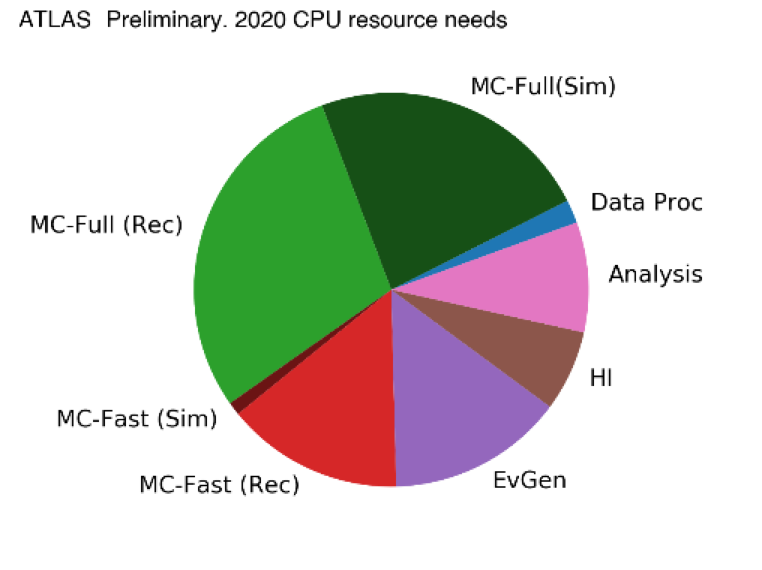
\includegraphics[width=0.70\textwidth]{figures/ATLASpreliminary2020CPUResourceNeeds.png}
    \caption{ATLAS CPU hours budgeted for various activities in 2020}
    \label{fig:Run3CPUbyActivity}
\end{figure}


ATLAS currently uses both Full simulation (FullSim based on G\textsc{eant}4) and Fast simulation (primarily parametrized calorimeter response) for physics results. Each physics analysis group evaluates the requirements for statistical and systematic precision for each physics sample that needs to be simulated. Based on these studies, physicists request some simulation samples with higher precision FullSim, and others with lower precision fast simulation. Reconstruction time for simulated events are currently similar for both simulation methods (but see FastChain discussion in next section). On average, currently about 50\% of all samples use FullSim. For the HL-LHC we aim to reduce this fraction to 25\%, thereby saving half of the CPU resources devoted to detector simulation at the HL-LHC. 

Besides reducing the fraction of events simulated with G\textsc{eant}4, we have an active R\&D program aimed at optimizing the CPU requirements of G\textsc{eant}4. Performance gains of ~20\% with no impact on physics performance have been already demonstrated and another ~20\% should be achievable.  The FullSim configuration for Run 3 will include the use of "Frozen Showers" in the forward region as in Run 1 and Run 2.

Reducing the fraction of MC simulated using FullSim requires analysers to be confident in using samples produced using fast simulation techniques in their analyses.  The agreement between full and fast simulation (and data) for key features of physics distributions has to be good enough that analyses are not biased.  In ATLAS this is mostly determined by the Combined Performance (CP) Groups who are responsible for producing the calibrations which allow comparison between data and MC.  The goal for Run 3 is for FullSim and fast simulation to agree to within uncertainties in the CP Group calibrations, so that the same calibrations can be used for all MC samples.  CP Group calibrations take a lot of person-hours to produce, so there would be reluctance to introduce an extra set of calibrations.

It should be noted that despite the goal of reducing the fraction of events simulated using G\textsc{eant}4 in Run 3, G\textsc{eant}4 will remain a critical part of our simulation strategy. It will be used to produce the samples used to tune parameterizations used by the fast simulation and will continued to be developed to give an improved description of interactions in the detector. A key improvement planned for Run 3 is to include energy deposits made directly by B's, D's and $\tau$ leptons, which in Run 2 were dealt with solely by the Generation step. This blurring of the line between Generation and Simulation will continue in Run 3 as G\textsc{eant}4 works to include b-physics in their physics lists.

For Run 3 ATLAS will combine hard-scatter and pile-up events at the digit (RDO) level.  The approach will be to make pre-mixed pile-up datasets by combining minbias events simulated by Geant4 and digitizing them together in the absence of a hard-scatter event. The pre-mixed pile-up RDO datasets will then be stored on the grid.  In the main production workflow hard-scatter events will be digitized then "overlaid" on top of a pre-mixed pile-up RDO event.  This process is considerably (quantify) faster than, and with much reduced I/O requirements compared to, pile-up digitization and scales much less steeply with pile-up luminosity.  As long as each pre-mixed pile-up RDO event can be used more than once then there is a reduction in resource requirements.  A strategy for how best to store and access the O(PB) pre-mixed RDO datasets will be developed over the next few months.  Another new issue for Run 3 is the variation of the beamspot size at the same time as $\langle\mu\rangle$ is varying.  The simplest way to deal with this is to have multiple (three?) sub-campaigns for each data period each simulated with a different beam spot width.  All but the last sub-campaign will look at beam conditions during the luminosity levelling regime, so $\langle\mu\rangle$ will be constant. The final sub-campaign will replicate the beam after levelling has finished and so will have a variable $\langle\mu\rangle$ value.
%\begin{itemize}
%    \item (shower libraries dead after Run 3)
%    \item implications on computing model.
%\end{itemize}
\subsection{Run 4 Strategy}
Run 4 analyses will need ten times more MC events than previous campaigns, so O(200) billion events. It will not be possible to produce this much MC using FullSim or even with Fast Simulation. For Run 4 ATLAS will need to switch to FastChain as the baseline simulation approach. For the simulation step, this involves using an ACTS-based fast Track simulation for the Inner Detector and FastCaloSim for the Calorimeter. Doing this will make the simulation time small compared to the reconstruction time, so further speed-ups to the MC production workflow will require reducing the reconstruction time (Add reference).  One possible idea is to use Trigger-like Algorithms to filter events prior to reconstruction, so that events which will never be used in analyses are not reconstructed (or written out). Another idea would be to use a strategy like Overlay, but to reconstruct the pile-up tracks in separate job, producing RDO-prime files containing pile-up tracks. These tracks could be copied through the overlay step. Reconstruction would then consist of running tracking for the hard-scatter, then combining the track collections and using the merged track collection as the input to the rest of the reconstruction.
Even if it is possible in principle produce the required sample sizes, they will still need to be stored somewhere. Current projections suggest that it will not be possible to store the required samples on disk.  Not storing intermediate file formats is a possible way to reduce the disk requirements.

\subsection{R \& D needed for Run 4} 
\begin{table}[htb!]
  \caption{Monte Carlo Chain CPU times in HS06~$\times$~seconds. Full Sim is Geant4+Frozen Showers in the FCAL. Fast Simulation is FastCaloSim V2 in the Calorimeter and G4 elsewhere. Full digi is digitizing hard-scatter and minbias hits together.
  MC Overlay is digitizing the hard-scatter and then combining with a pre-digitized zerobias event. Fast Chain is simulation using FATRAS in the Inner Detector, FastCaloSim V2 in the Calorimeter and Geant4 in the Muon System; digitizing the hard-scatter and combining with a pre-digitized zerobias event, where ID Tracking has already been performed. Standard reconstruction is assumed, except for the Fast Chain case, where ID Tracking is performed for the hard-scatter only.}
  \label{tab:SimCPU}
  \centering
  \begin{tabular}{|c||c|c|c||c||c|} \hline
    scenario & Hard-scatter & Hard-scatter & Hard-scatter & Background & Hard-scatter \\
             & EVNTtoHITS & HITStoRDO & RDOtoESD & from table 2 & Total \\ \hline
    Full sim $+$ & 5684 & $\langle\mu\rangle=$140: 3317         & 402        & 23 & 9403 \\
    Full digi &   & $\langle\mu\rangle=$200: 4233         & 584        & 33 & 10534 \\   
    Full sim + & 5684 & $\langle\mu\rangle=$140: 183          & 402        & 92 & 6351 \\
    MC Overlay &   & $\langle\mu\rangle=$200: 202 & 584        & 121 & 6611 \\   
    Fast sim + & 1137 & $\langle\mu\rangle=$140: 183          & 402        & 92 & 1814 \\
    MC Overlay &   & $\langle\mu\rangle=$200: 202 & 584        & 121 & 2044 \\
    Fast Chain + & 114 & $\langle\mu\rangle=$140: 183          & 278        & 95 & 669 \\
    MC Overlay &   & $\langle\mu\rangle=$200: 202 & 370        & 126 & 811 \\ \hline
    \end{tabular}
    % Sim + Digi numbers taken from results of running in 21.9 provided by Markus
    % Reco numbers taken from table in section 6.5
    % Newer G4 version will be faster
    % Assuming MC Overlay time is negligible (need a better estimate).
    % From the Overlay note: For the standard method, at μ=70 the CPU time required is 7.5 times larger than for μ=10. For the MC-overlay method the increase in CPU time is only 20% when increasing μ from 10 to 70. Extrapolating this to μ=200 the CPU time is 20 times higher for the standard method and < 2 times higher for the MC-overlay method.
    % Assuming G4+FCS is 5 times faster than full G4
    % Assuming that FATRAS (ID) + FCS + G4 (MS) is 10 times faster than G4+FCS
    % Assuming that running ID Tracking on zero bias will make reco tracking time negligible (probably wrong)
\end{table}

\begin{table}[htb!]
  \caption{Monte Carlo Background costs per hard-scatter in HS06~$\times$~seconds. Re-use factors are the number of times these events are re-used later in the workflow. The assumption here is that the size of the minbias HITS and zerobias RDO samples will scale with $\langle\mu\rangle$ }
  \label{tab:SimCPU}
  \centering
  \begin{tabular}{|c||c|c|c|c|c|} \hline
             &  Production & Re-use & $\langle\mu\rangle$ & No. used per & Cost per \\ 
             &  [HS06s] & factor & & Hard-scatter & Hard-scatter [HS06s]\\ \hline
    Low pT minbias & 2120 & 1867200 & 140 & 5446 & 6\\
    Low pT minbias & 2120 & 1867200 & 200 & 7780 & 9\\
    High pT minbias & 5787 & 4800 & 140 & 14 &  17 \\
    High pT minbias & 5787 & 4800 & 200 & 20 &  24 \\
    Zerobias RDOs & 3317 & 48 & 140 & 1 & 69 \\
    Zerobias RDOs & 4233 & 48 & 200 & 1 & 88 \\
    Zerobias RDOs + ID Tracks & 3441 & 48 & 140 & 1 & 72 \\
    Zerobias RDOs + ID Tracks & 4447 & 48 & 200 & 1 & 93 \\ \hline
    \end{tabular}
  

    % Sim + Digi numbers taken from results of running in 21.9 provided by Markus
    % Reco numbers taken from table in section 6.5
    % Newer G4 version will be faster
    % Assuming MC Overlay time is negligible (need a better estimate)
    % Assuming G4+FCS is 8.5 times faster than full G4
    % Assuming that FATRAS (ID) + FCS + G4 (MS) is 10 times faster than G4+FCS
    % Assuming that running ID Tracking on zero bias will make reco tracking time negligible (probably wrong)
\end{table}
%\begin{itemize}
%    \item Justify sample sizes required (disk requirements)
%    \item Nature of the samples: CP samples, background samples.
%    \item {\it \color{blue}  Number of fast simulation flavours: multiple flavours require %multiple validations/calibrations. OTH multiple flavours can be optimized for different analyses.
%    \item Run 4 baseline: FastChain}
%\end{itemize}
Detector simulation is projected to continue to be one of the main consumers of CPU resources in Run 4 and beyond. ATLAS is eager to collaborate with international efforts to parallelize G\textsc{eant}4 detector simulation. Preliminary evaluations and prototyping in the areas of G\textsc{eant}4 EM physics and particle transport indicate that a substantial speedup in G\textsc{eant}4 event throughput is possible on a time scale of 5-10 years.

Development will be required to produce MC Overlay events at $<\mu>=200$. MC Overlay events are currently produced using the pile-up digitization workflow used in Run 2. This approach is not compatible with AthenaMT running. Most likely this approach will be used for Run 3, but it will not be suitable for the high $<\mu>$ values expected in Run 4. This will involve sharing background minbias events between multiple threads.

Finally a rich ATLAS-wide R\&D program in collaboration with others is aimed at developing fast, high-fidelity detector simulation using generative neural network models. Depending on the fidelity achieved by these models in simulating tails in the detector response, another factor ~2x may be saved in CPU resources for simulation by producing fewer events simulated with full G\textsc{eant}4.





%\begin{itemize}
%    \item Strategy to store O(200B) MC events, 
%    \item Continue investigating role of GANs. Discuss training samples size.
%    \item External R\&D needed: parallelising Generators and Geant4
%\end{itemize}
\subsection{Discussion on number of events needed}

\subsection{Trigger simulation}
The Run~4 trigger system consists of a hardware and software trigger system~\cite{ATLAS-TDR-29}. The hardware trigger is simulated using dedicated algorithms that strive to perform a bit-wise correct emulation of the trigger decision. The majority of the system consists of FPGA-based electronics that can be simulated on a regular CPU without much performance penalty.

The Hardware Track Trigger (HTT) on the other hand uses a custom associative memory chip to perform massively parallel pattern look-ups for finding track candidates.
Regular ATLAS simulation and reconstruction will use the parameterised fast simulation (FastHTTSim), which applies smearing of offline/truth/HLT track parameters, with negligible need of resources. 
The resource intensive full HTT simulation (HTTSim), will only be used for the following use-cases: performance studies at high pile-up in a limited $\phi$ slice (1/32); estimation of fake and dataflow rates with high-pileup samples; parameterisation of the fast simulation using single-muon events. The generation of constants for the pattern-matching and track-fitting (HTTSimGen) requires high statistics samples of simulated single-muon events. 

The required CPU resources for one production cycle are summarised in Table~\ref{tab:httsim}. A new production will be required when data-taking conditions (e.g. tracker alignment, LHC interaction region) change significantly and is estimated to about two cycles per year. Additional cycles will be needed during the commissioning phase of the project. HTT validation may also need additional samples to study tracking performance in dense environments.

The samples sizes and event processing times are conservative estimates with very large uncertainties derived from previous FTK studies. Further detailed studies are needed to get better estimates on samples sizes and processing times. To reduce the required resources, alternative processing methods are under consideration, like the usage of GPUs or the possibility to process simulated data directly on the HTT hardware system at Point-1. 

\begin{table}[h]
    \centering
    \begin{tabular}{|l|l|l|r|r|r|}
      \hline
      use case                  & sim. type &  event type & events/cycle & HS06/event & HS06/cycle \\
      \hline
      ATLAS simulation          & FastHTTSim  & any         &  any   & negligible & neglible \\
      Performance high-PU       & HTTSim  & min-bias   & 1 M  & 1.2 M/32 & 37500 M\\
      Fake and dataflow  high-PU & HTTSim  & min-bias   & 50 k   & 1.2 M & 60000 M\\
      Parameterization          & HTTSim  & single muons    & 50 M   & 100 & 5000 M\\
      Generation of constants  & HTTSimGen & single muons   & 1 B   & 135 & 135000 M\\
    
      \hline
    \end{tabular}
   \caption{Extrapolations of CPU resources for global HTT during regular data-taking per production cycle (see text). A CPU reduction of 20\% per event is expected if only regional HTT is simulated.}
    \label{tab:httsim}
\end{table}

%\subsection{Impact}
%The results of these R\&D efforts will have a 2-16X impact on the resources needed for MC simulations at the HL-LHC, as described in this document.


\section{Reconstruction}
% Markus, Ed, Peter L, Caterina
%% {\it\color{red} Section Editors: Markus, Ed, Peter L.}
\label{sec:reco}

Dealing with the increased event complexity from unprecedented levels of pile-up, reaching an average of 140 simultaneous proton-proton collision ($\langle\mu\rangle$) during Run~4 and up to 200 in the subsequent Runs, poses a challenge in particular to the offline event reconstruction and to the physics object identification. At the same time, it will be vital for the ATLAS Phase-2 programme that the physics performance of the reconstructed objects will be preserved wherever possible improved w.r.t. the Run~2/3, despite the increasing level of pile-up expected for Phase-2.
%
\begin{table}[htb!]
  \caption{The CPU required in HS06~$\times$~seconds to reconstruct data 2018 events at an average of 90 pile-up from a dedicated high pile-up run when using the current software reconstruction software. Compared are the results for track reconstruction, muon and calorimeter reconstruction, combined reconstruction and monitoring using the Run~2 software release.}
  \label{tab:RecoCPU}
  \centering
  \begin{tabular}{|c|c||c|c|c|c||c|} \hline
    Detector & $\langle\mu\rangle$ & inner    & muon spectrometer & combined       & monitoring & total \\
             &                     & tracking & and calorimeter   & reconstruction &           &        \\ \hline
    %% old data 17: Run~2    & 50                  & 337      & 31                 & 24            & 25        & 29   & 462  \\ \hline
    %% master nightly Feb.2 on data 18 Raw to all, HS06 scaling of the machine is 22.
    Run~2    & 90                  & 1137     & 149               & 301            & 106       & 1693  \\ \hline
    %% Phase-2  & 140                 & 124      &                   &                &           &       \\
    %%          & 200                 & 214      &                   &                &           &       \\ \hline
    \end{tabular}
\end{table}

Estimates based using the current Run~2 software to reconstruct raw data from a dedicated run taken in 2018 with an average pile-up of 90, as shown in Table~\ref{tab:RecoCPU}, indicate that for the current detector and software all aspects of event reconstruction require significant CPU resources to deal with the increased event complexity, with the inner track reconstruction dominating in CPU needed because of its pronounced scaling with pile-up. ATLAS is undertaking a major detector and software upgrade program to facilitate the required physics performance improvements and at the same time to help reduce the CPU requirements for event reconstruction:
%
\begin{itemize}
    \item 
    The design of the Phase-2 tracker upgrade (ITk)~\cite{ATL-PHYS-PUB-2019-014} has been optimised not only for physics performance, but at the same time the design aims to minimise CPU for reconstruction at an average of 200 pile-up. The five layer ITk Pixel Detector with its ring design will facilitate fast track seeding and finding approaches.
    \item
    ATLAS carried out a prototype study~\cite{ATL-PHYS-PUB-2019-041} to demonstrate that classical CPU based algorithmic approaches can exploit the ITk detector design for a fast track reconstruction to resolve the CPU problem, at the expense of some limited loss in physics performance.
    \item
    ATLAS initiated the ACTS~\cite{acts} open source project to develop the next generation tracking software in a common cross experiment project, with the aim to use ACTS to achieve both, CPU reduction and excellent physics performance, for the Phase-2 reconstruction. Moving to ACTS will not only address the challenge of ITk reconstruction, but at the same time it will help reducing the CPU for other aspects of reconstruction, like particle flow or muon reconstruction.
    \item
    An equally important aspect of the ATLAS Phase-2 reconstruction strategy is a strong programme of algorithm R\&D to improve all aspects of event reconstruction, to further reduce the CPU needs and to maximise physics performance. This includes a broad set of R\&D initiatives of applying Machine Learning and novel data science inspired algorithmic approaches to reconstruction, as well as R\&D on exploiting co-processors (i.e. GPUs) for offline event reconstruction. 
\end{itemize}

%%%%%%%%%%%%%%%%%%%%%%%%%%%%%%%%%%%%%%%%%%%%%%%%%%%%%%%%%%%%%%%%%%%%%%%

\subsection{The Tracker Upgrade and the Fast Track Reconstruction Strategy for Phase-2}
\label{sub:ITKFastTrack}

%
\begin{figure}[htb!]
  \centering
  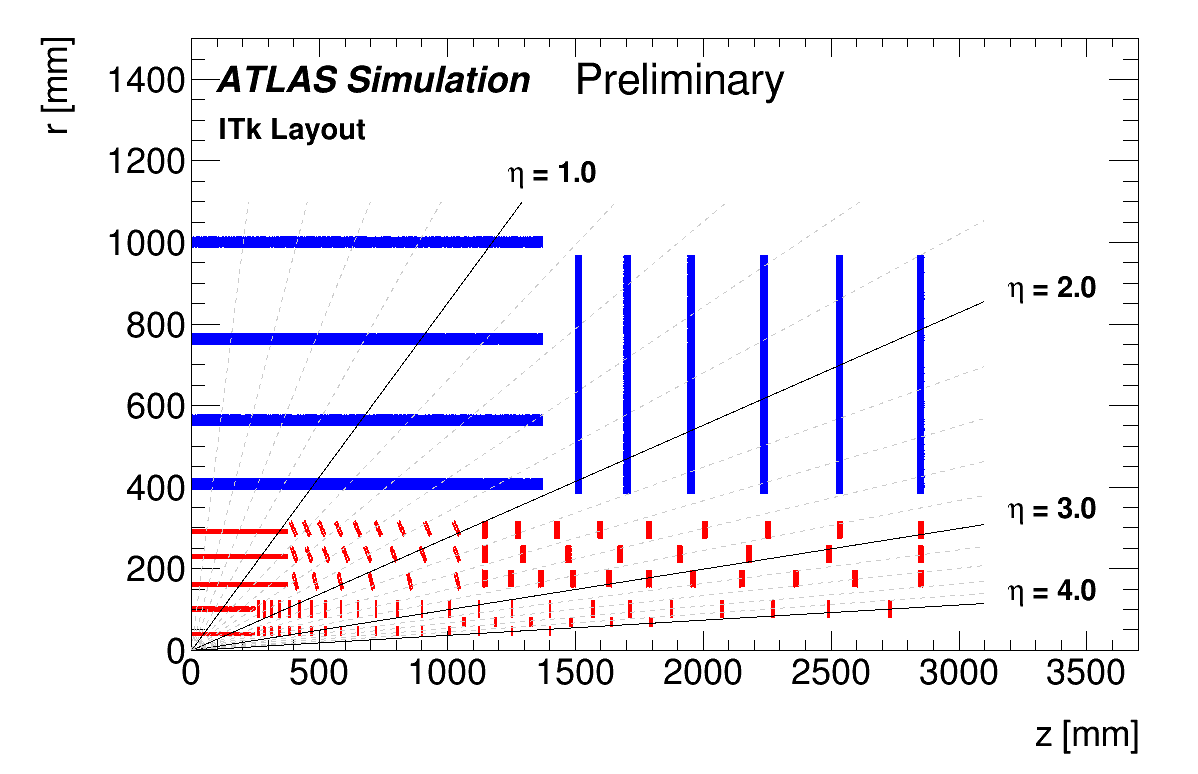
\includegraphics[width=0.51\textwidth]{figures/HitsRZ_Half_ITkLayout}
   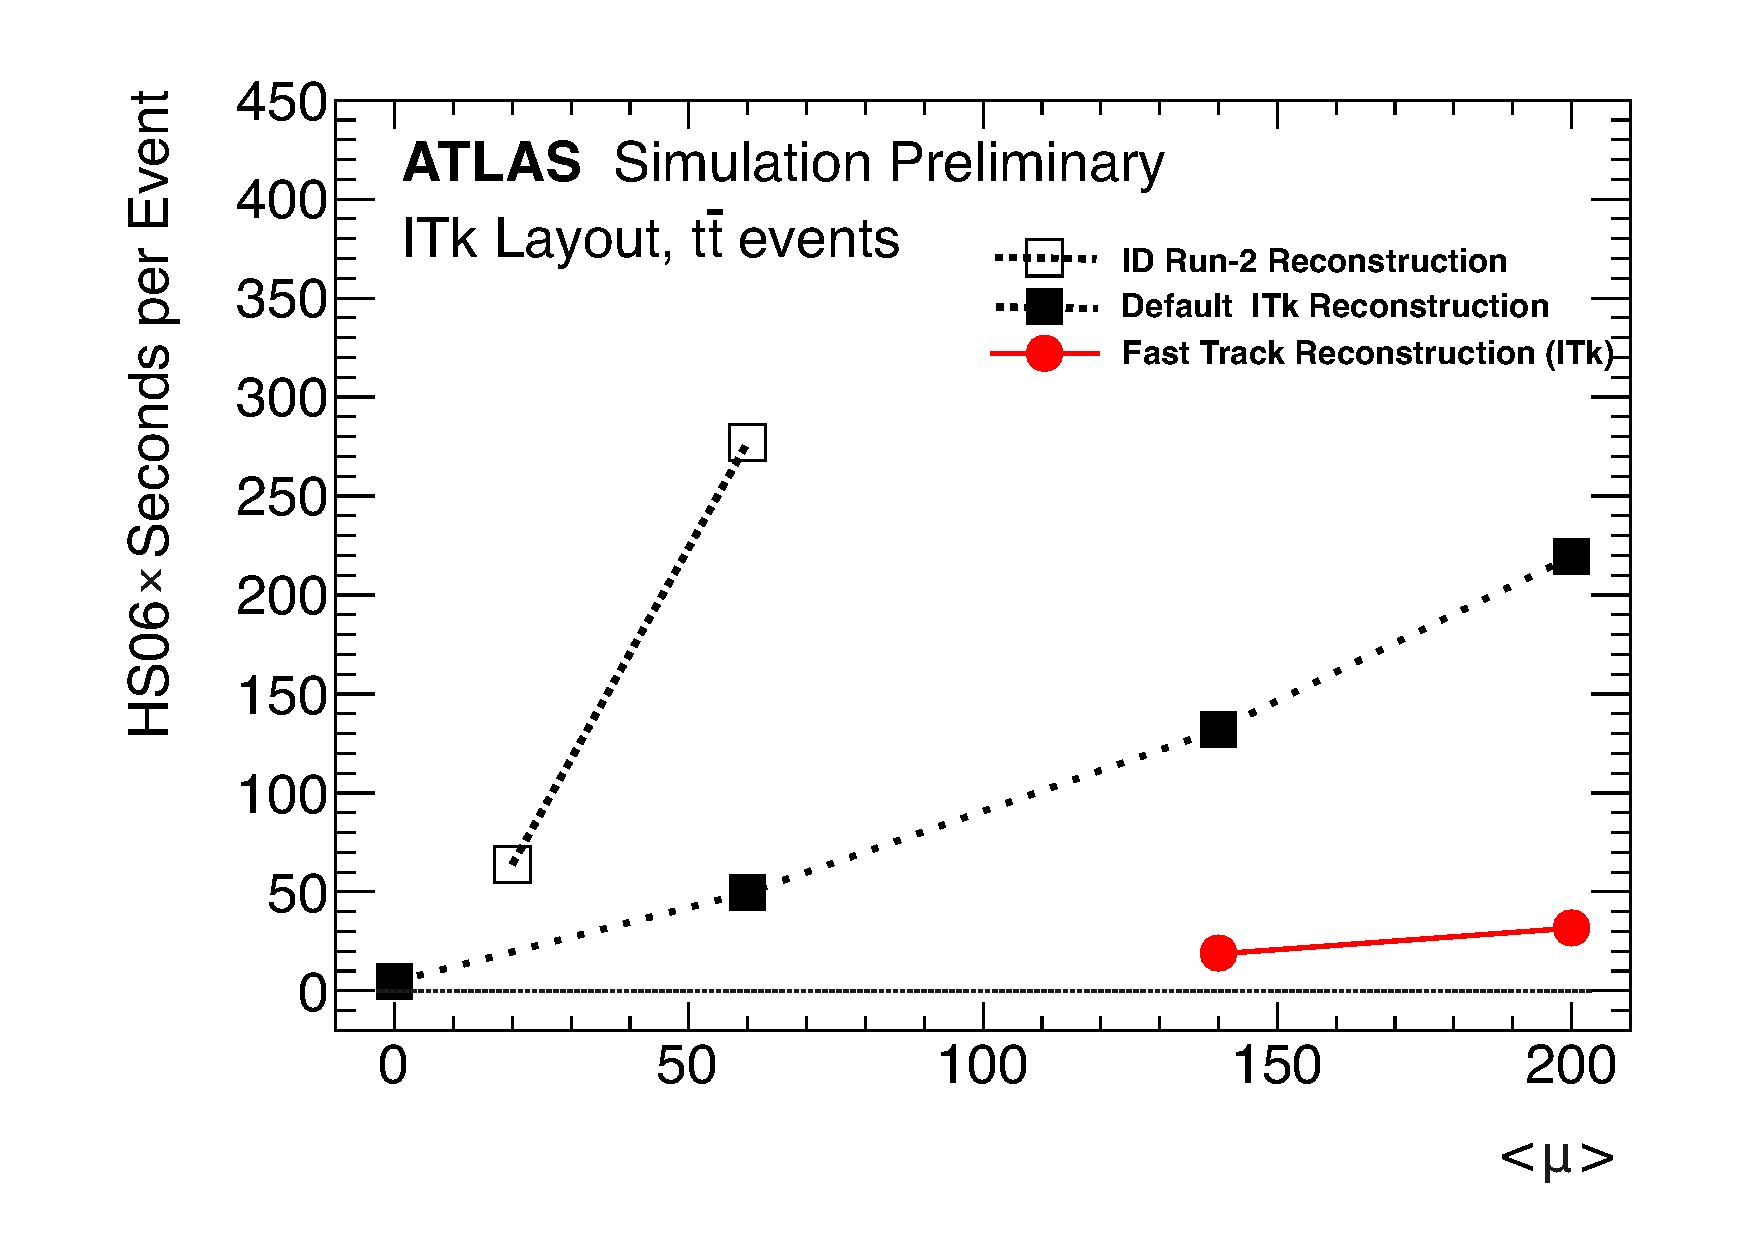
\includegraphics[width=0.47\textwidth]{figures/Timing_fast_ITkLayout_Run2}
  %% 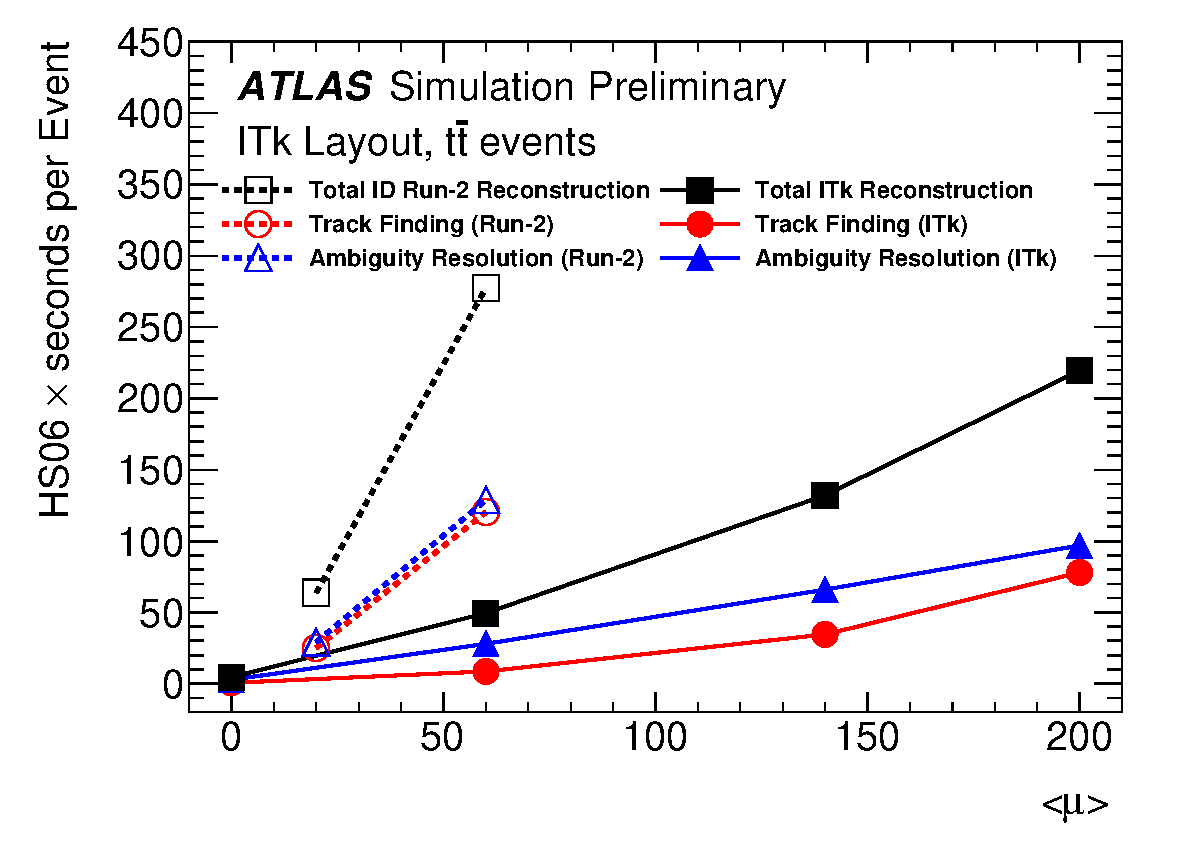
\includegraphics[width=0.47\textwidth]{figures/Timing_ITkLayout_Run2}
  \caption{{\bf Left:} A schematic layout of the ``ITk Layout'' with a five layer Pixel Detector (red) surrounded by the Strip Detector (blue). Only the positions of the active sensors are shown. {\bf Right:} The CPU required in HS06~$\times$~seconds to reconstruct a $t\bar{t}$~event in the current ID and the ITk at different levels of $\langle\mu\rangle$. Standard Run~2 reconstruction was used for the current ID, while for the ITk results are shown using the Run~2 software (black line) and the fast track reconstruction (red). Figures taken from References~\cite{ATL-PHYS-PUB-2019-014} and \cite{ATL-PHYS-PUB-2019-041}.}
  \label{fig:ITkandCPU}
\end{figure}

Figure~\ref{fig:ITkandCPU} illustrates the design of the ITk and the results of the fast track reconstruction study. The left plot shows a schematic $R-z$ view of the ITk detector layout that will consist of a five layer pixel system covering 8 units in $\eta$, surrounded by a four layer double sided strip detector with small stereo angle. The new tracking detector has been optimised for 200 pile-up, with an improved granularity, a constant hit coverage, a reduced material budget in the active tracking volume and a sensor placement that also aimed at minimising CPU for pattern recognition. The right plot shows the CPU required for track reconstruction as a function of average pile-up for the current ID and the ITk. Using the Run~2 tracking software to reconstruct the current ID, a strong scaling in CPU is observed between $\langle\mu\rangle = 20$ and $60$. Shown on the same plot is the CPU required by the Run~2 tracking code to reconstruct the ITk with an average event pile-up of up to 200. The ITk allows to significantly reduce the CPU to 124 and 214 HS06~$\times$~seconds, respectively, for an average pile-up of 140 and 200. At the same time the ITk will improve in physics performance compared to the current ID~\cite{ATL-PHYS-PUB-2019-014}.
%
\begin{table}[htb!]
  \caption{The CPU required in HS06~$\times$~seconds to reconstruct $t\bar{t}$ Monte Carlo events with $\langle\mu\rangle = 140$ and 200 in the ITk. Listed are the results for the different reconstruction steps using the current Run~2 software and the fast ITk track reconstruction. An Intel Xeon E5-2620v2 was used with 2.1~GHz and six physical cores per CPU. The CPU time is multiplied with the HS06 factor of 17.8 for single thread running. The Table is taken from Reference ~\cite{ATL-PHYS-PUB-2019-041}.}
  \label{tab:FastTrackCPU}
  \centering
  \begin{tabular}{|c|c||c|c|c|c|c||c|} \hline
   $\langle\mu\rangle$  & Tracking & Byte Stream                  & Cluster     & Space  & Si Track & Ambiguity  & Total \\
                        &          & Decoding                     & Finding     & Points & Finding  & Resolution & ITk   \\ \hline
   \multirow{2}{*}{140} &  Run~2   & \multirow{2}{*}{1.2$^{(*)}$}  & 17.1        & 6.0    & 41.1     &  58.2      & 124 \\
                        &  fast    &                              & 4.5         & 0.9    & 12.4     &  -         &  19.0 \\ \hline
   \multirow{2}{*}{200} &  Run~2   &  \multirow{2}{*}{1.6$^{(*)}$} & 26.3        & 8.6    & 85.8     &  92.0      & 214 \\
                        &  fast    &                              & 6.3         & 1.2    & 22.6     &  -         &  31.7 \\ \hline
  \end{tabular} \\
  $^{(*)}$ {\tiny Scaled from Run-2, see text.}
\end{table}

ATLAS has undertaken a study~\cite{ATL-PHYS-PUB-2019-041} to demonstrate the possible CPU performance improvements achievable by optimising the Run~2 track reconstruction techniques for Phase-2 levels of pile-up. The two tracking algorithms requiring the largest fraction of CPU are the Silicon Track Finding and the Ambiguity Resolution. The Ambiguity Resolution takes about 60\% of the total CPU time to apply the final precise track fit and to handle the pixel cluster splitting in dense environments using a Neural Network~\cite{Aad:2014yva}. For the purpose of this prototype study, the Ambiguity Resolution algorithm is omitted from the reconstruction chain. Instead, a tighter track selection and precise cluster calibrations are applied already at the stage of the Silicon Track Finding to remove duplicate tracks and fakes.
% The Silicon Track Finding algorithm now also makes use of the precise cluster calibrations, while still using an approximate material model and approximations in the cluster corrections.
The five layer Pixel Detector covers the full range of $|\eta| < 4$ such that the seed finding could rely only on pixel hit combinations, leaving out the strip seed iteration.
% For the purpose of this study the option for the recovery for Bremsstrahlung was temporarily disabled in the Silicon Track Finding.
In addition, technical improvements were applied e.g. to the strip and pixel clustering and space point formation to better optimise the software for Phase-2 levels of pile-up.

Table~\ref{tab:FastTrackCPU} summarises the CPU times for using both the Run~2 and the fast tracking code reconstruction for reconstructing the ITk. The fast version of Silicon Track Finding is approximately eight times faster for $\langle\mu\rangle = 140$ and 200, respectively. The fast track finding is about a factor 1.8 faster for the $\langle\mu\rangle = 140$ sample, compared to the $\langle\mu\rangle = 200$ sample. Adding the CPU needs for the Cluster Finding and the Space Point Finding algorithms, the total CPU requirement for the fast ITk track reconstruction becomes 19 and 31.7 HS06~$\times$~seconds for $\langle\mu\rangle = 140$ and 200, respectively. The left plot of Figure~\ref{fig:ITkandCPU} shows the result for the fast reconstruction in red.
%
\begin{figure}[htb!]
  \centering
  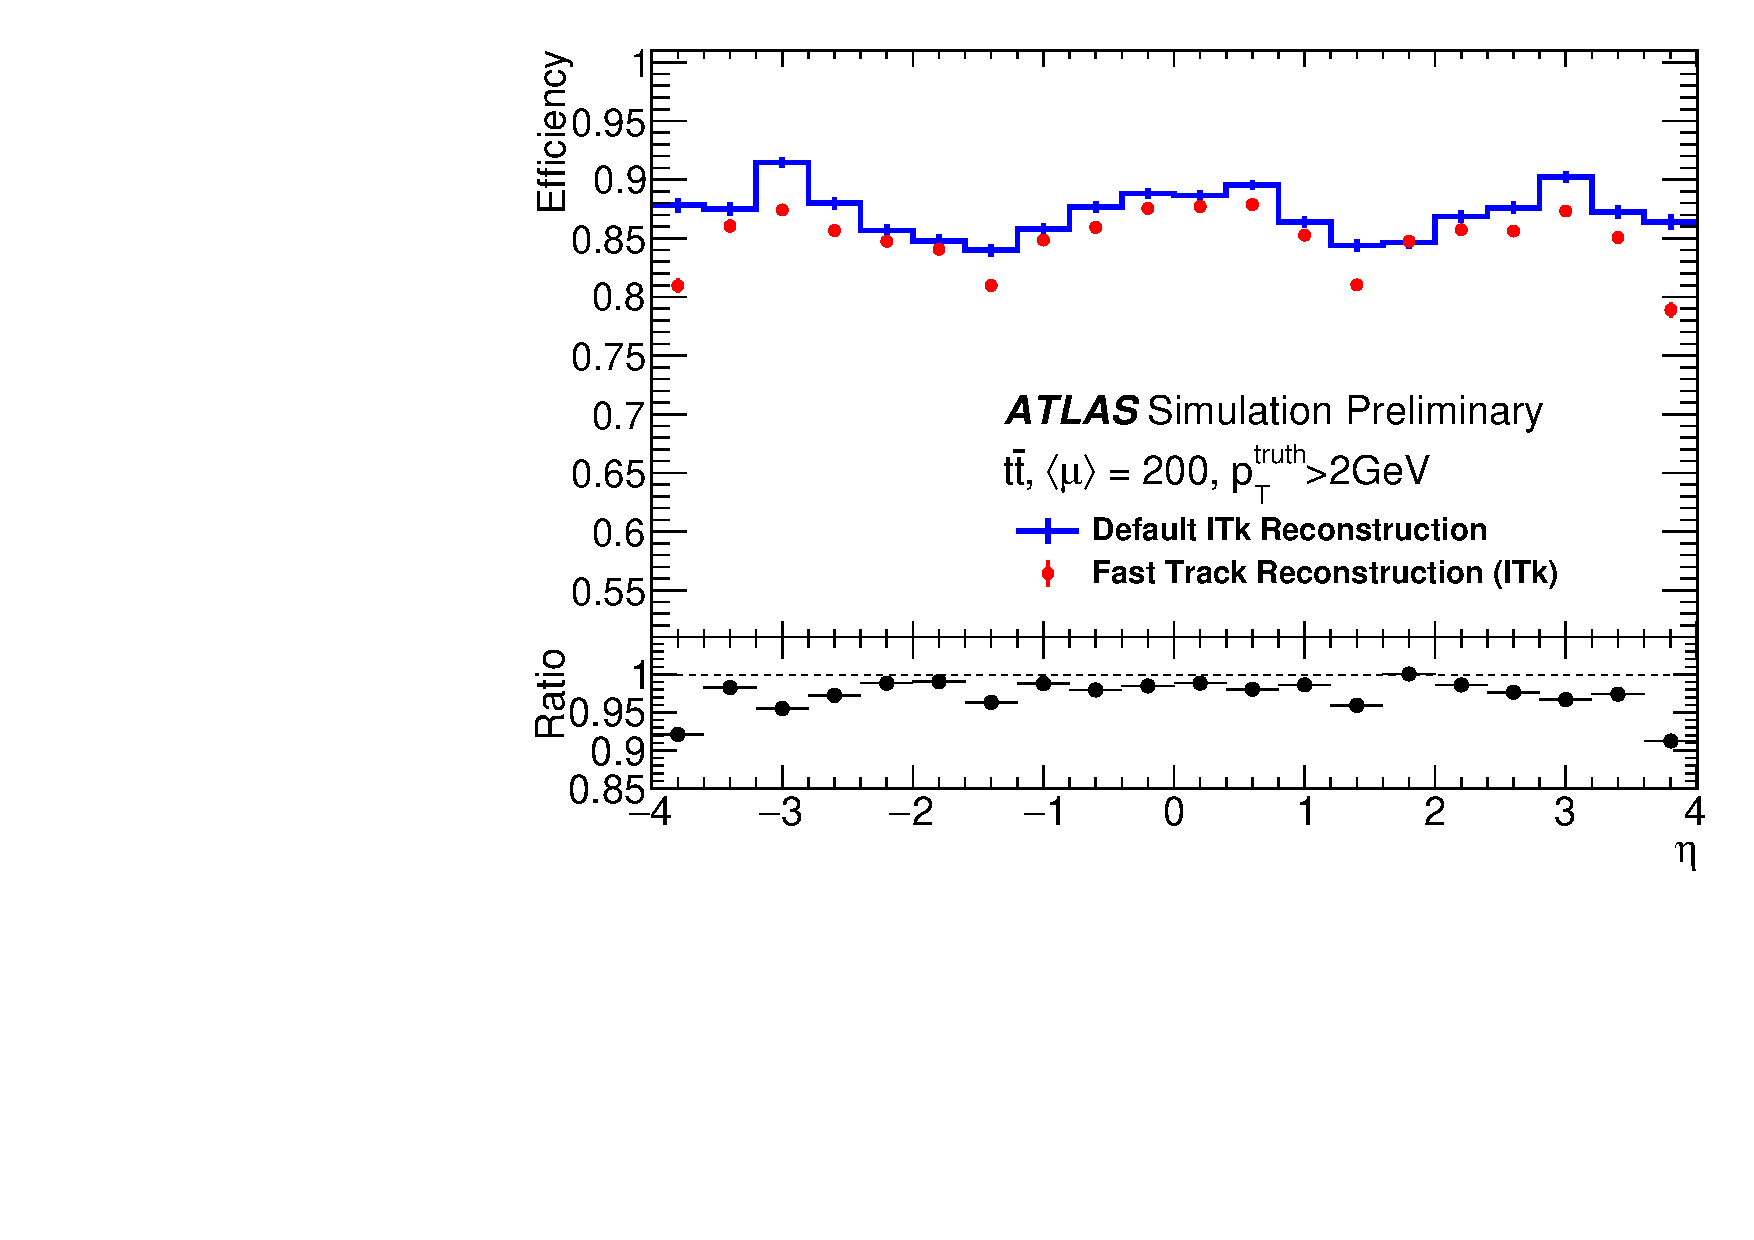
\includegraphics[width=0.48\textwidth]{figures/efficiencyEtaCombined}
  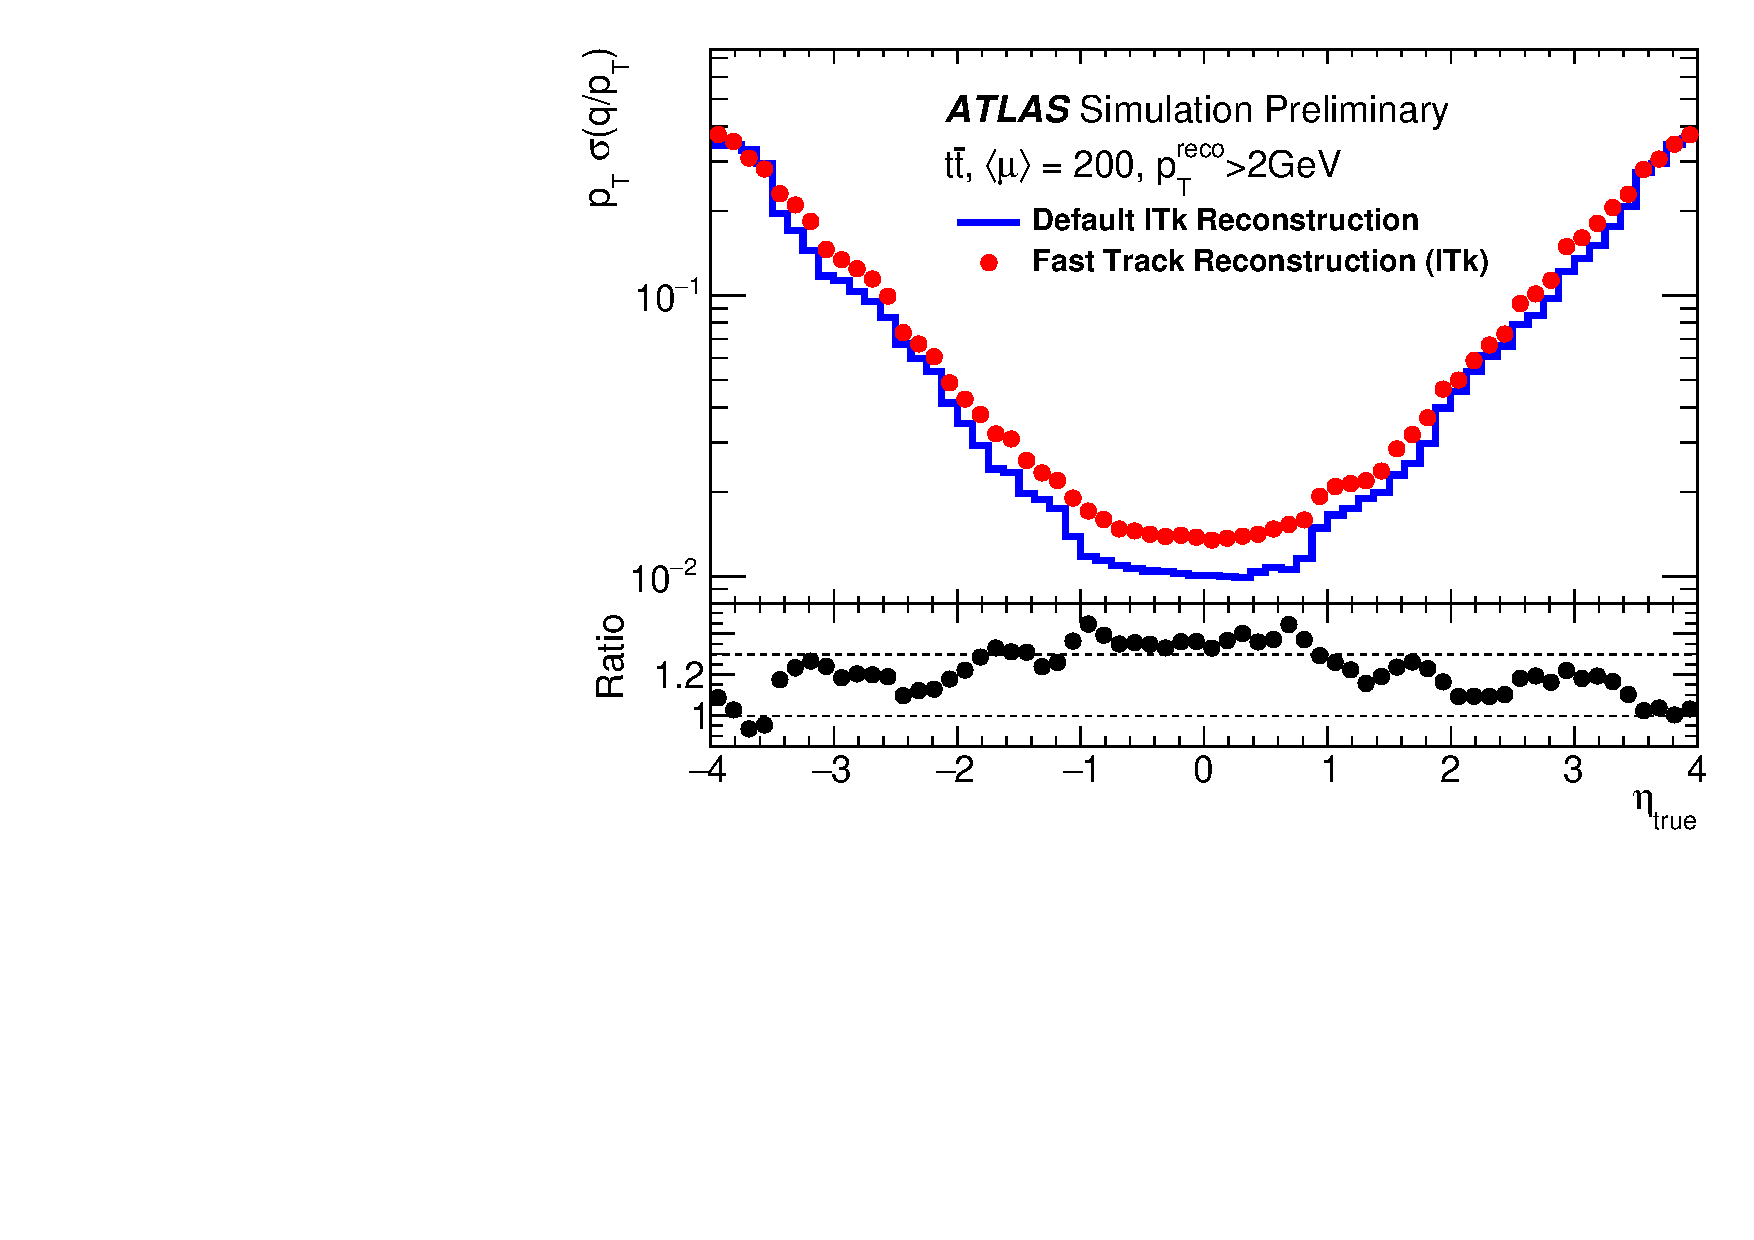
\includegraphics[width=0.50\textwidth]{figures/QoPEtaRatio}
  \caption{{\bf Left:} Tracking efficiency as a function of $\eta$ for the fast and the default ITk reconstruction. {\bf Right:} Relative transverse momentum $p_T$ as a function of $\eta_{true}$. Samples of $t\bar{t}$~events are used with $\langle\mu\rangle = 200$. A $p_T$ cut of 2~GeV is used for the generated particles, to avoid turn-on effects. The ratio is given by the efficiency for the fast reconstruction divided by the efficiency for the default reconstruction.}
  \label{fig:FastTrackingPerf}
\end{figure}

As expected because of the preliminary nature of this study, the fast ITk track reconstruction yields some loss in physics performance due to approximations made. Figure~\ref{fig:FastTrackingPerf} shows the loss in track reconstruction efficiency and in momentum resolution when comparing the fast and the default reconstruction on a sample of $t\bar{t}$~events with an average of 200 pile-up. A more detailed assessment of the tracking performance can be found in Reference~\cite{ATL-PHYS-PUB-2019-041}. This study demonstrates that it is possible to address the ITk track reconstruction problem for Phase-2 levels of pile-up using current tracking techniques on a classical CPU.

%%%%%%%%%%%%%%%%%%%%%%%%%%%%%%%%%%%%%%%%%%%%%%%%%%%%%%%%%%%%%%%%%%%%%%%

\subsection{The ATLAS Reconstruction Software Upgrade using ACTS}

The goal of the ATLAS Phase-2 software upgrade programme is not only to achieve the ultimate physics performance, but at the same time to modernise the software technology and to make best use of coming and future processing technologies. Technical performance improvements are expected in the area of event data model, data structures and data locality, in mathematical library optimisation and in the algorithms used for reconstruction.
%
\begin{comment}
\begin{figure}[htb!]
  \centering
  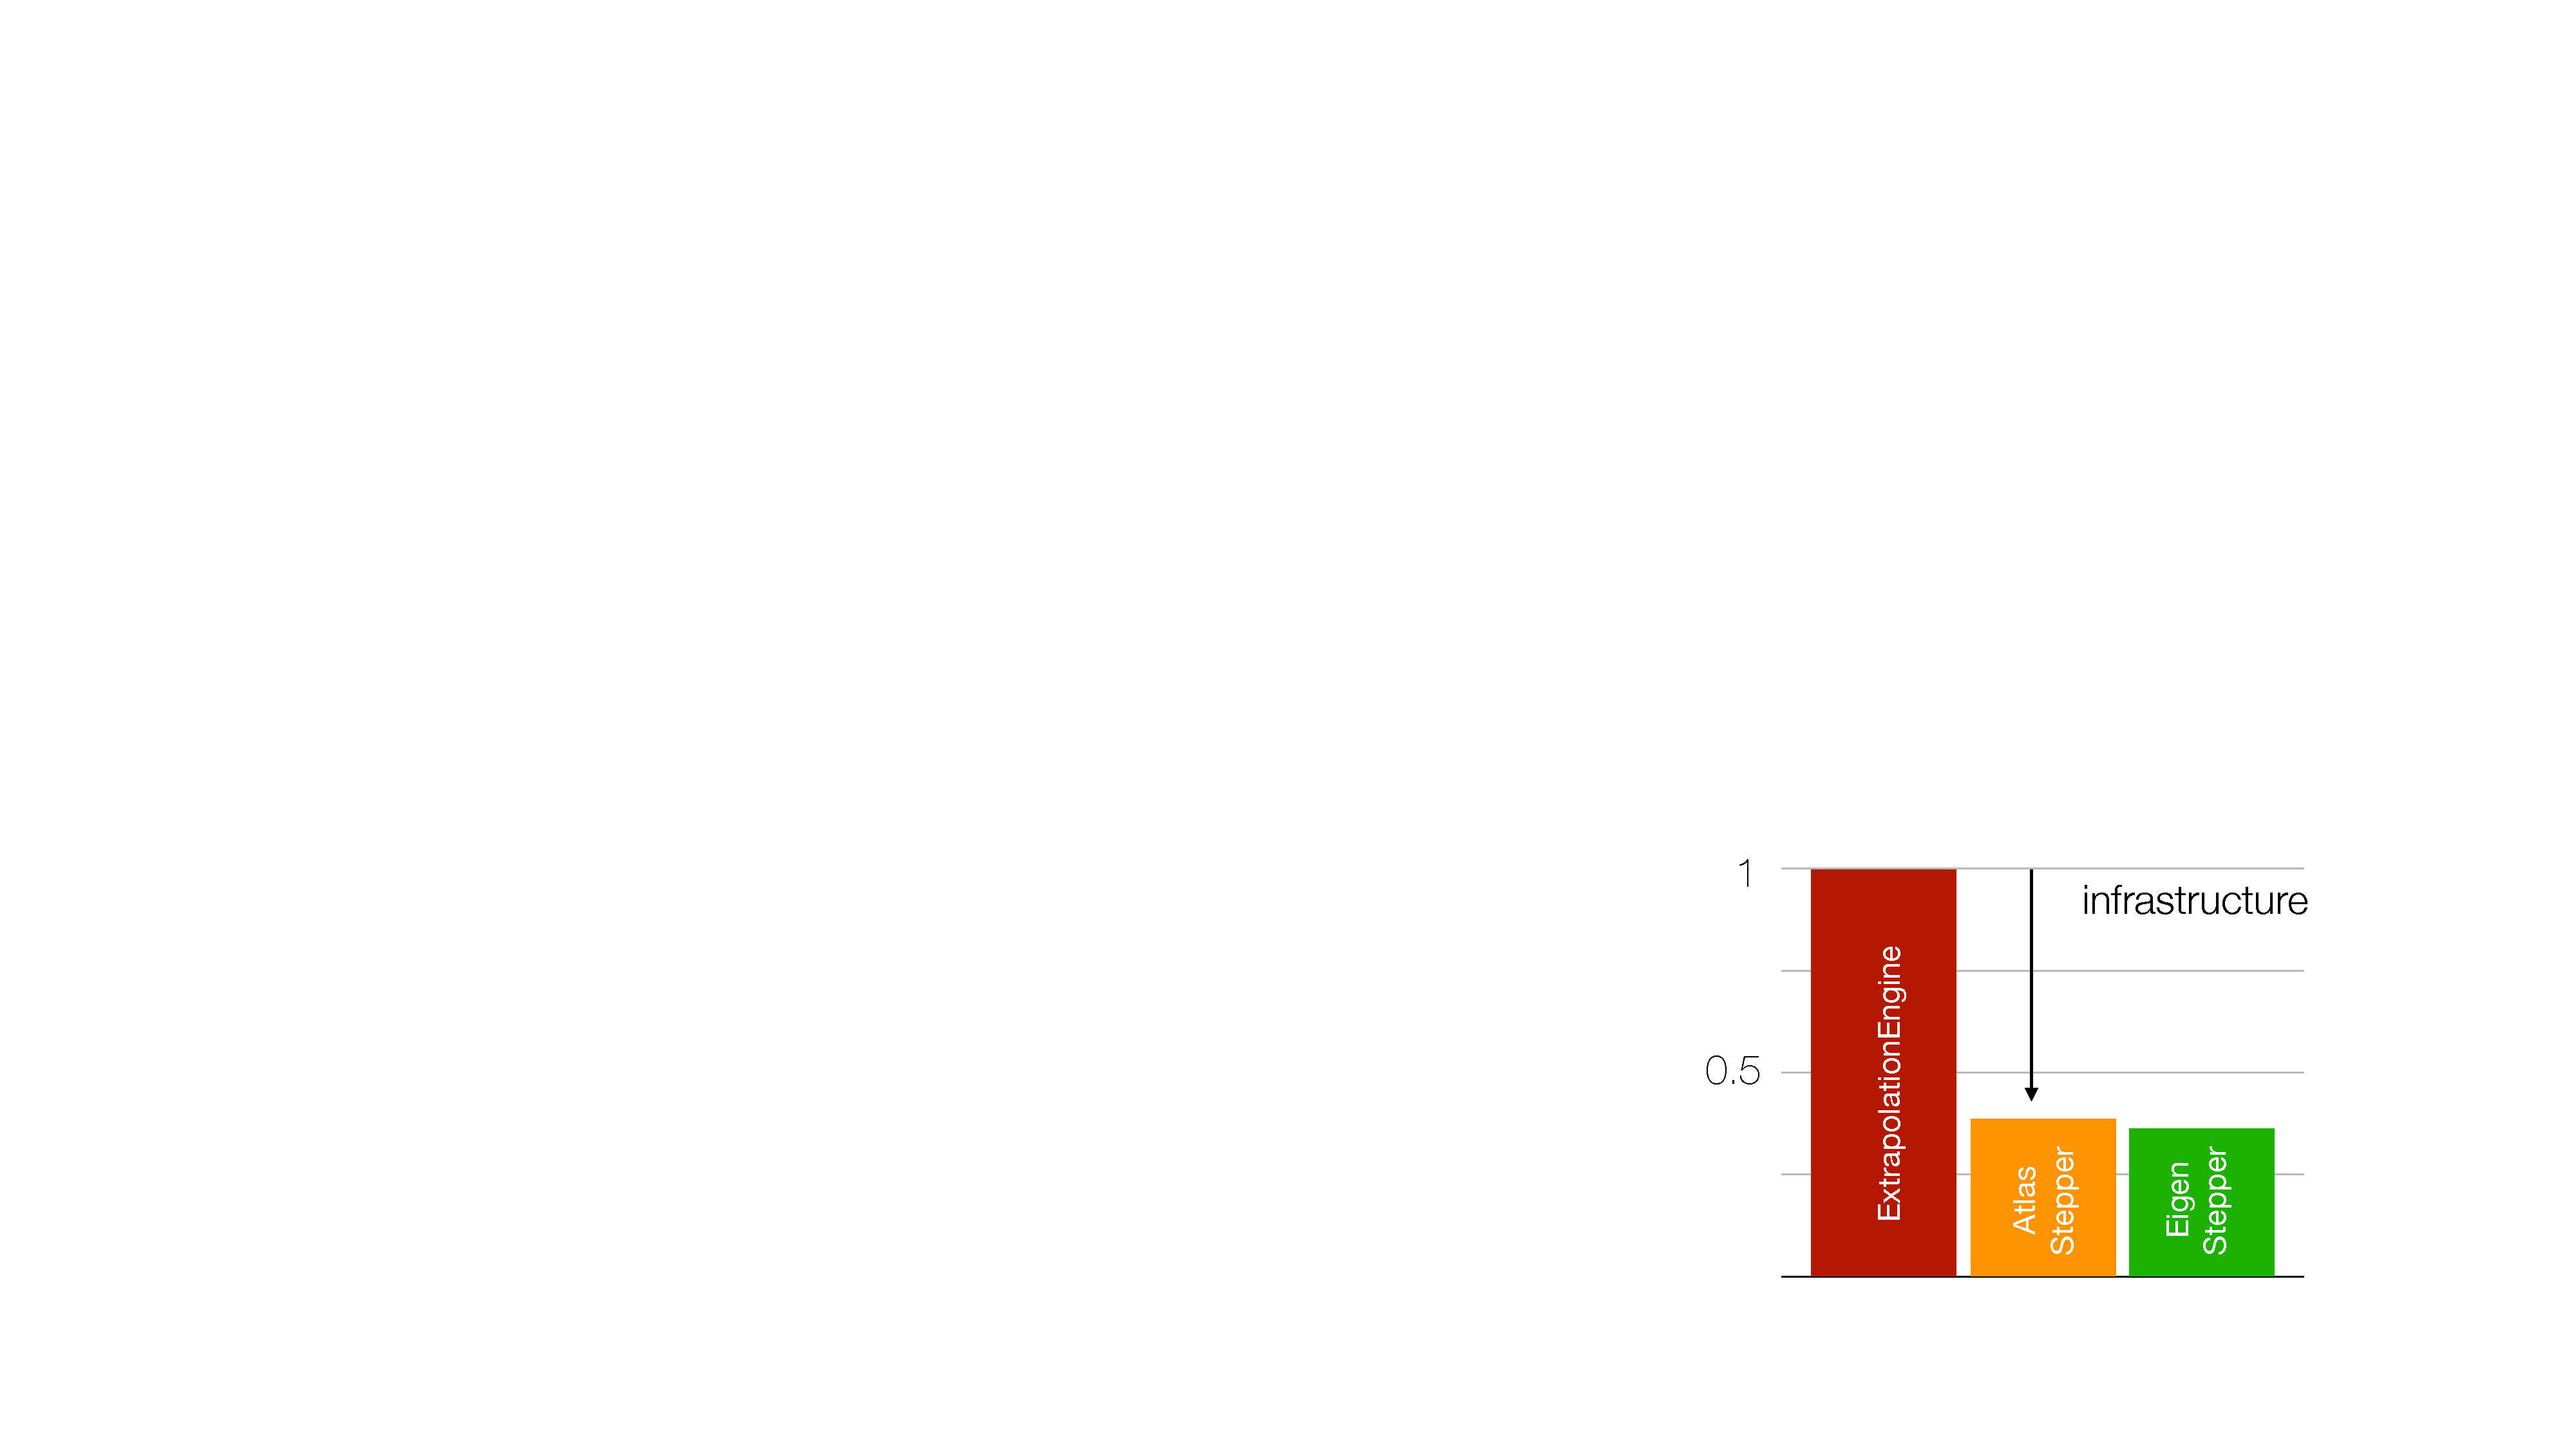
\includegraphics[width=0.40\textwidth]{figures/ACTSStepper}
  \caption{Relative timing comparison between two magnetic field stepping tools with the current ATLAS default extrapolation engine. Figure is taken from Reference~\cite{AndiCHEP2018}.}
  \label{fig:ACTSPerf}
\end{figure}
\end{comment}

ATLAS has launched the ACTS project~\cite{ACTS} as an open source tracking software project within the HEP community at large. The ACTS tracking software suite has been designed from the start for multi-threaded event processing and having data locality in mind. It significantly simplifies the technical overheads w.r.t. the current ATLAS tracking software and is aimed at a better utilisation of vector processing capabilities of modern CPUs. ATLAS is currently in the process of integrating the first functional components of the ACTS suite for the Run~3 event reconstruction. 
% Figure~\ref{fig:ACTSPerf} show an example for the technical performance improvements expected using ACTS compared to the current offline tracking software. The plot compares the relative speed for two of the the magnetic field integration stepper implemented in ACTS with the corresponding field integration using the ATLAS extrapolation engine. Figure is taken from Reference~\cite{AndiCHEP2018}.

Replacing the current suite of tracking tools use in the current Run~2/3 reconstruction with ACTS will result in significant CPU gains across the application, from the Inner Detector and Muon Spectrometer tracking, to all combined reconstruction using charged tracks. An important deliverable of the ACTS projects is a fast combinatorial Kalman filter, that will be used in the fast Silicon Track Finding to recover the full physics performance. The same Kalman filter will be used in the Ambiguity Resolution together with the Neural Network cluster splitting to recover from physics performance losses of the fast ITk track reconstruction prototype in the core of dense jets.
% Monte Carlo studies show that with this strategy the Ambiguity Resolution will only be applied to less than 5\% of the track candidates.
% The Bremsstrahlung option of the ACTS Kalman filter will used to recover inefficiencies for electron track in the fast Silicon Track Finding, adding a few \% to the total CPU budget for ITk reconstruction.

The Muon Spectrometer and combined muon reconstruction will benefit from the improved technical performance of the ACTS tracking tools. The new ACTS Gaussian Sum filter implementation is foreseen to replace the current software in the combined electron reconstruction and the ACTS extrapolation code will be used for the particle flow algorithm combining calorimeter and tracking information for jet finding and missing energy reconstruction. Primary vertex reconstruction, conversion finding, $tau$ reconstruction and $b$-tagging will be based on the ACTS vertexing package. The reconstruction of the Phase-2 High Granularity Timing Detector (HGTD) will use the ACTS software for associating timing hits to forward tracks.

%%%%%%%%%%%%%%%%%%%%%%%%%%%%%%%%%%%%%%%%%%%%%%%%%%%%%%%%%%%%%%%%%%%%%%%

\subsection{Optimising Reconstruction for Phase-2 Levels of Pile-up}

The physics performance of all object reconstruction and identification at Phase-2 needs to match and where possible exceed the current Run~2 performance, if ATLAS wants to reach its physics goals. All algorithms in the reconstruction chain need to be fully optimised for high pile-up, taking into account the CPU resource limitations. Technical software improvements, like the introduction of ACTS for the full reconstruction chain, are essential to meet the goals.

ATLAS is running an ambitious development programme for improved and novel algorithmic approaches for all detector and combined reconstruction aspects. Examples are optimised strategies for combined muon reconstruction that improve the acceptance for soft muons or handle more gracefully events with hadronic showers leaking into the Muon Spectrometer.

Calorimeter reconstruction is expected to not be affected by the high luminosity, both in terms of CPU time consumption and memory usage and both for data and Monte Carlo simulations.
This is due to the particular reconstruction algorithms for this detector system, which are described in detail in Ref. \cite{Aad:2016upy}. As for Run~1 and Run~2, they start from the whole (fixed size) list of individual signals and yield a stable average number of final signal objects (topological cell clusters), rather independent of the luminosity. 
While the existing calorimeter reconstruction algorithms are not expected to change significantly,
possible reconstruction performance improvements and computing resource reductions are under study. 
In particular, these include the formation and calibration of the topological cell clusters using machine learning techniques (see Reference~\cite{PERF-2014-07}).

New particle flow \cite{PERF-2015-09} objects will be introduced that support a more efficient extraction of overlapping and shared signals in complex Phase-2 events and thereby allow to extract efficiently an unambiguous event representation. Improved techniques for pile-up rejection will be developed for all combined reconstruction, exploiting the detailed particle flow information, the improved tracking performance with the ITk and the timing information from the HGTD in the forward. 

%%%%%%%%%%%%%%%%%%%%%%%%%%%%%%%%%%%%%%%%%%%%%%%%%%%%%%%%%%%%%%%%%%%%%%%

\subsection{Streamlining Reconstruction for Unconventional Signatures of New Physics}
\label{sec:reco-unconvsig}

One of the primary goals of the (HL-)LHC physics programme is the search for New Physics. Several models for New Physics give rise to experimental signatures involving meta-stable particles. A possible signature are charged particles decaying within the tracking system, leading to signatures of so-called disappearing tracks. Meta-stable heavy particles, as e.g. predicted in some R-parity violating SUSY models, may give rise to displaced production vertices for charged particles that tend to have large impact parameters and are only measured in the outer layers of the tracking system.

During Run~2 ATLAS was using a so-called pixel tracklet reconstruction step run after the primary track finding to identify candidates for disappearing tracks. A dedicated trigger stream was used to pre-select candidate events for CPU intensive reconstruction of tracks from displaced vertices. A significant fraction of the total CPU for data reconstruction was spend on the processing of the additional stream of selected displaced vertex candidate events, which also required significant additional data storage capacities. ATLAS aims to simplify the reconstruction strategy for such unconventional signatures for Phase-2. It is planned to integrated the pixel tracklets as a second track selection strategy in a unified single path Silicon Track Finding step, minimising the additional CPU resources needed. Because of the significant differences between the detector signatures of primary charged particles and those for displaced tracks, a second path of the Silicon Track Finding will be required. To limit the amount of CPU resources needed, this second path will only be applied to events pre-selected by dedicated trigger signatures.

Integrating the track reconstruction for unconventional signatures into the data processing chain will increase the CPU requirement for Tier-0, but the total amount of CPU required for reconstruction will be significantly reduced and the data processing model will be simplified, also reducing the amount of storage needed during Phase-2.

%%%%%%%%%%%%%%%%%%%%%%%%%%%%%%%%%%%%%%%%%%%%%%%%%%%%%%%%%%%%%%%%%%%%%%%

\subsection{Prospects for the technical Performance of the Phase-2 Reconstruction}

Two scenarios for the technical performance of the Phase-2 reconstruction were studied. The results of the current Run~2 based software for Phase-2 reconstruction are used as a baseline. Future improvements from the fast ITk reconstruction, the introduction of ACTS, the improvements in muon and calorimeter software, as well as in combined reconstruction, are expected to lead to significantly lower CPU resource requirements as a result of the Phase-2 reconstruction software upgrade programme.
%
\begin{table}[htb!]
  \caption{Prospects for CPU required in HS06~$\times$~seconds for reconstruction at different levels of average pile-up for Phase-2. Shown are the numbers for a $t\bar{t}$ Monte Carlo sample as measured for the current Run~2 based reconstruction software. In brackets the goals of the software upgrade programme are shown exploiting the Fast Track Reconstruction, ACTS and further technical and algorithmic optimisation of all aspects of the reconstruction software chain. Results for MC truth processing and framework overheads for I/O (etc.) are not included.}
  \label{tab:Phase2CPU}
  \centering
  \begin{tabular}{|c||c|c|c|c|c||c|} \hline
    \,\,\,\,\,$\langle\mu\rangle$\,\,\,\,\, & primary tracking & unconventional & calorimeter,      & combined       & monitoring & total reconstruction \\
                        &                  & signatures     & muon spectrometer & reconstruction &            &       \\ \hline
    140                 & 124 (35) & - (25)         & 157 (85)          & 51 (35)        & 70 (35)    & 402 (215)  \\
    200                 & 214 (50) & - (30)         & 176 (95)          & 94 (70)        & 100 (50)   & 584 (295) \\ \hline
    \end{tabular}
    % default is measured in 20.20 on ttbar
    % the assumption is that ACTS and technical updates with gain 30% in muon tracking, drop MuGirl
    % calo reco unchanged
    % 30% on egamma, jets, met. tau etc unchanged
\end{table}

Table~\ref{tab:Phase2CPU} summarises the technical CPU requirements for the baseline scenario using the current Run~2 based reconstruction software and, in brackets, when extrapolating the expected software and algorithmic improvements from the Phase-2 software upgrade programme. The evolved scenario includes the CPU for the reconstruction of unconventional signatures in the normal processing chain. The budget for offline monitoring on real data for Phase-2 is assumed to be 100 HS06~$\times$~seconds and 50 for the improved scenario, for running at 200 pile-up. At 140 pile-up 70 and 35 is assumed, respectively.

The software upgrades, if successful, may lead to more than a factor two speed improvement, compared to the current Run~2 software, also incorporating the processing of events for unconventional signatures. Track reconstruction will still account for a significant fraction of the overall reconstruction time, with a larger number of other reconstruction steps contributing at a similar level to the total CPU needed.

%%%%%%%%%%%%%%%%%%%%%%%%%%%%%%%%%%%%%%%%%%%%%%%%%%%%%%%%%%%%%%%%%%%%%%%

\subsection{Algorithm R\&D, Machine Learning and co-Processors}

The offline reconstruction will need to be adapted to the rapid evolution in software and processing technologies. Over the past years Machine Learning and other Data Science inspired techniques have been developed that promise to boost the physics performance for all aspects of event reconstruction. Techniques like similarity hashing, metric learning or graph networks are being investigated as alternatives~\cite{InstutitePascalTracking} to the classical track reconstruction techniques. For Phase-2 such novel techniques may be applied in the offline reconstruction or trigger context, also with the goal improve the technical CPU performance. It is therefore vital that ATLAS continues to further invest in such R\&D.

Most current and next generation HPC systems will provide the majority of their computing power in form of GPU co-processors. Online reconstruction for trigger processing can potentially benefit from deploying GPU co-processors in the trigger farm of the experiment. While all GPU co-processors offer large parallel processing capabilities, the model for programming those devices significantly differs from classical X86 processors. Supporting a heterogeneous set of co-processor technologies is therefore also a software development challenge. ATLAS is currently exploring different technologies like CUDA, OneAPI, Kokkos and alpaka for the integration of co-processors in its offline event processing framework ATHENA~\cite{ATHENA}. The aim is to develop tools for efficient offloading of algorithmic code onto different co-processors using the same code base and to minimise the need of vendor specific software development for the applications itself.

The model of using GPU co-processors for event reconstruction depends on the sharing of workloads in the application. Offloading of a few algorithmic kernels, that otherwise would require a large fraction of the overall CPU budget, is not possible for the ATLAS Phase-2 event reconstruction. As can be seen in Table~\ref{tab:Phase2CPU}, the improvements of the fast ITk track reconstruction will yield to a much more even distribution of CPU needed for the different algorithmic parts of the event reconstruction chain. Packages like ACTS and new ATLAS algorithmic code developed for Phase-2 are being designed from the start to better support parallel processing. Memory models required for efficient processing on GPU co-processors will also help improving data locality for X86 processing. Novel Machine Learning and Data Science inspired algorithmic approaches for event reconstruction are also evaluated for the ability to exploit GPU co-processors. The exact model for a more fine-grained offloading of algorithmic workloads onto co-processors is yet a subject of intensive R\&D. The ATLAS Phase-2 computing model extrapolations for offline reconstruction are therefore based on X86 processing and no assumptions are made on additional gains from particular co-processing and related software technologies.

\section{Visualization}
% Riccardo Bianchi <riccardo.maria.bianchi@cern.ch>, Sergei Chekanov <chekanov@anl.gov>

% \subsection{Introduction}

Interactive visualization is a key tool in High Energy Physics experiments \cite{ref:atlas-event-visualization}. Not only does interactively visualizing data from particle collisions help in understanding the physics involved in the interactions between fundamental particles; it is also a necessary tool for a number of different tasks in the HEP workflow, from detector development to simulation, reconstruction, physics analysis, and outreach \cite{ref:atlas-public-ed}. %Visualization tools are also used to prepare high-quality and engaging event displays for papers, conferences, announcements, and press releases \cite{atlas-public-ed}. 
A faithful and uncluttered visualization of the physics objects is essential %to offer 
to give physicists the right tools to inspect, verify, and debug their data. Physics objects---like tracks, vertexes, hits, or calorimeter cells---have to be clearly rendered, to let users distinguish the interesting ones even in a view where a large number of them are shown. In addition to that, tools to accurately handle them and to navigate through the view have to be offered, to let users focus on specific objects or on certain areas. 
Moreover, interactive tools like object selection, highlighting, and filtering must be accurate enough to let users pick the right item, to get detailed information about it or to set selective filters.
%On top of that, users have to be able to set cuts on different variables, to 

In Phase-2, as explained in Section~\ref{sec:reco}, the foreseen increase in the number of simultaneous proton-proton collisions will yield a related increase in the event complexity. The number of physics objects to reconstruct will increase enormously and, with that, the number of objects to be visualized. Thousands of superimposed tracks  and hundreds of very close vertexes will be visible in any given event, besides the other objects. The development of new visualization software  techniques, besides the upgrade to modern technologies, will be vital to properly show such a large number of actors and to correctly interact with them. Without that, it will be very hard, if not impossible, for physicists to visually investigate collision data effectively to debug their collection, reconstruction, and analysis.


% In the following of this section, a list of the improvements and developments needed to meet the requirements of Run III and Run IV will be given, with a strategy plan and a timescale.

\subsection{Improvements in the Run III timescale}

A certain number of software and technology updates foreseen for Run IV are planned to be started in a timescale compatible with Run III. That will prepare the path to the further software development for Run IV, while easing visualization in Run III already. 



%\subsection{Improvement of the visualization of physics objects}
\paragraph{Improving the visualization of physics objects}

As explained in Section \ref{sec:reco-unconvsig}, a variety of models for New Physics within the (HL-)LHC physics program involve signatures with meta-stable particles and displaced vertexes. 
Currently, focus has been put in the visualization of the primary vertexes; secondary and displaced vertexes miss a dedicated set of visualization features to show the decay of meta-stable particles in detail and properly isolate it from the environment. Also, visualization of tracks produced at the displaced vertex should be rendered differently and isolated on demand, for detailed inspection. Those new  features will be crucial to check the selection algorithms used for signatures involving meta-stable particles.
Different types of particle jets also play a key role in many physics models for New Physics. For that, a detailed visualization of the calorimeter activity is essential and dedicated views and tools are needed to let ATLAS physicists verify the jet reconstruction algorithms and the analysis selection cuts. 
New "Lego" plots and cluster visualization features will be added to the ATLAS event display tools, VP1~\cite{ref:vp1-web} and Atlantis~\cite{ref:atlantis-web} respectively. 


%\subsection{Improvement of the Online Event Display for data taking}
\paragraph{Improving the Online Event Display for data taking}

The "Online Event Display" system running in the ATLAS control room is an essential tool in the context of Data Preparation. It gives the ATLAS shift crew a prompt visual feedback about the data taking. Anomalies or large asymmetries in the distribution of physics objects are quickly spotted, triggering further inspection. The system runs a dedicated reconstruction chain over the experimental data as soon as they are collected and event displays are produced and stored for further inspection. 
Currently, the system offers 2D views of the collected data, overlaid to a simplified geometry of the detector, created with Atlantis~\cite{ref:atlantis-web}. It is considered important, however, in the context of Data Preparation needs, to update the system with the features offered by another ATLAS event display, VP1~\cite{ref:vp1-web}, to produce 3D views of data, overlaid to an exact copy of the detector geometry, directly taken from the experiment's software framework. This will let ATLAS scientists get a prompt feedback about the correct behaviour of the different parts of the detector. %Also, the additional application will provide additional 3D views to the shifters, with tools useful to visualize problematic data in details.
For that, the setup of the the Online Event Display system will be updated, to produce filtered data for both the event display applications. Also, pre-defined views will be defined for both applications, to support the activities of the ATLAS control room crew.



\subsection{A better visualization of geometry volumes for Detector Description}

As explained in Section \ref{sec:detdescr}, the geometry of the ATLAS detector in Run IV will be dramatically different from the current one. Thus, major detector development work is foreseen in the next years to write and update the detector description.% for Run IV; and the plan is to have tools which let developers work outside the experiment's framework Athena as much as possible.  
To support that, major software development will be needed in the visualization of detector geometry. 

A large number of new developments are foreseen for Run IV in the context of Detector Description visualization. Work is currently ongoing to create visualization tools tailored to geometry volumes. Our vision is to have standalone, interactive tools to inspect, query, and explore the geometry information tree and to handle geometry volumes. For that, a number of new features will have to be developed, such as a dedicated geometry browser to quickly see the structure of the detector description tree in details; interactive tools to quickly get information about a subset of the tree or a single volume on request, ideally both from a list of volumes and by clicking on the 3D view; the ability to filter on volumes' properties (names, materials, shapes, and so forth) to selectively visualize parts of the geometry; the development of a new visualization schema to be able to visualize both mother and children volumes at at he same time; the possibility to interactively modify the shapes in the 3D view and save their representation into a file. %Even if planned for Run IV, the first implementations of the above mentioned tools will be used in Run III as well. 
The new tools will play a key role in the implementation and debug of the new detector description, letting developers develop it in an efficient workflow with fast visual feedback.

% \begin{itemize}
%     \item interactive volume filtering
%     \item interactive selection of volumes
%     \item better model view (Browser) and further interaction between the model view and the 3D objects
% \end{itemize}




\subsection{New rendering techniques for very dense environment}

    

In Run IV, the increased pile-up will cause the production of large number of physics objects. The extremely large number of vertexes and tracks will make the visualization of those events hard; in addition to that, picking and selecting the right object in such a dense environment will be extremely difficult, making the interaction of physicists with the physics objects cumbersome. 

The graphical rendering of those objects will play a major role. In such dense events, tracks and vertexes should be rendered with selective techniques, to highlight the interesting ones, or the one on the front of the current view, while hiding or dimming the others. Similar techniques should be applied to effectively display vertexes, when a large number of them are present in the view. Our current visualization tools are not able to do that. 

In other fields of research, like brain studies and medicine, visualization techniques have evolved to let scientists effectively visualize objects in very dense environments. The visualization of those objects shares many of the challenges we will have to face to dynamically and selectively visualize tracks in HL-LHC events. 
The study of modern rendering techniques and their implementation in our workflow will require the adoption of modern graphics libraries and technology. Thus, development work will be needed to replace the graphics engines used in our current visualization tools with more modern incarnations.
In parallel, new selection tools will have to be developed, to let physicists correctly identify and interactively pick the right object from the busy environment.

The new tools will be critical to help physicists leverage the ATLAS discovery potential. Without those, it will be very hard to by visually check reconstruction algorithms and physics signatures in busy event data from HL-LHC collisions.



\subsection{Standalone visualization tools and new technologies}


Our current tools follow two approaches: either they are run inside the experiment's framework (VP1~\cite{ref:vp1-web}) to be able to access data directly, but with the disadvantage of having to run on supported platforms and being limited in the use of the software libraries from the experiment's software stack; or, they are standalone programs (\textit{e.g.}, Atlantis~\cite{ref:atlantis-web}) making use of data exporters to get a copy of the data, but with the need of re-running the export step every time new data or are needed or new selection cuts need to be applied to those.

Following the recommendations from HSF~\cite{ref:hsf-cwp-viz}, we will shall explore the possibility of decoupling the visualization of the experimental data from their retrieval and handling.
A server-client approach will let us keep the ability of accessing and querying data directly from the experiment, while being able to run our visualization tools on many platforms, explore new technologies (like web-based 3D rendering, or Virtual and Augmented Reality) without being limited by the experiment's needs in terms of stability of the software stack, and leverage the potential of the visualization pipelines supported by modern graphics hardware (GPUs). In addition to that, the new architecture will let us use modular, common packages from other HEP experiments and co-develop them (as emphasized in the aforementioned HSF white paper). 
Some exploratory work has been started already, to develop standalone visualization tools accepting streamed event data, based on web technologies (Phoenix~\cite{ref:phoenix-web}, started in ATLAS and then developed with contributions from other LHC experiments under the aegis of HSF). 
Major design and development work will be needed to develop a client-server pipeline.

The effort put in the development of the new architecture will return in larger simplicity and flexibility, both in terms of visualization software development and maintenance for the future of the ATLAS experiment.



\section{Analysis model}
% Lukas, Alison, Gordon

%\begin{itemize}
%    \item do we need any hard numbers beyond per-event size of %PHYS(LITE)? Target Event Processing Rate? 
%    PHYS: 50kb/event (currently 38 kb/event but missing some trigger %info and maybe other stuff)
%    PHYSLITE: 10 kb/event
%\end{itemize}

%Probably need to condense, for me main points for R4 are

%\begin{itemize}
%\item PHYS/PHYSLITE
%\item Integration into wider data science 
%\item Data Access 
%\item Interactive Analysis at HL-LHC scale
%\item (Analysis Automation)
%\end{itemize}

%Open Q:
%\begin{itemize}
%\item what about DAST/WLCG obv will evolve do we discuss it? AL: not %sure we should
%\item epxect accelerators  to be useful (e.g. github/hepaccelerate) AL: %Yes but can we say anything other than this?
%\end{itemize}

\subsection{Introduction}

While the vast majority computational resources at the LHC are spent on preparing reconstructed data and simulation datasets, a large fraction of human resources is spent on the analysis of the data collected by the experiment to produce physics results. It is imperative that the Analysis Model is conducive to a streamlined workflow which is easily usable to a typical analyst, with particular focus on enabling easy access to students at all levels. 
In light of the data volumes expected at the HL-LHC, an evolution of the current data reduction workflow~\cite{Derivation System} that consolidates the generation of  calibrated event data for analysis is important. In the baseline analysis model, the HL-LHC sees the full deployment and adoption of of the new data formats introduced during Run 3. In addition, on the timescale of the HL-LHC, the tool-chest accessible to physicists will broaden as industry tools for large scale data analysis develop and are incorporated into the HEP ecosystem. The analysis model must therefore serve both traditional and modern analysis tools. While these are not 'baseline', the early adoption of industry-standard tools should be encouraged and should replace traditional tools during Run 4.

\subsection{Analysis Data Formats}


A core recommendation of the AMSG-3 Task Force\cite{amsg3} is the introduction of two new common, data formats, {\sc DAOD\_PHYS} ($\sim$ 50kb/event) and {\sc DAOD\_PHYSLITE} ($\sim$ 10 kb/event). 
While Run 2's introduction of a centralized data reduction format (the Derivation Framework) was successful, a significant overlap in the derivations defined across the various analysis groups is observed. This motivated the common {\sc DAOD\_PHYS} format as a way to reduce disk space usage. This format is designed to include sufficient event data to perform final object calibration, though those object calibrations will not yet be applied.
On the other hand, the light-weight {\sc DAOD\_PHYSLITE} format will be a centrally produced data format for events in which all 'object' calibrations are already applied. To that end, the `CP Algorithms' maintained by the Analysis Model Group and the performance group, provide standard building blocks.
The goal of these data formats is to cover the needs of 'most' (~80\%?) ATLAS data analyses.
The remaining analyses will be served using custom derivations and (DRAW) filters with every effort made to reduce the number of processed events.

In the current computing model, a large amount of disk space, and significant human time, is typically taken up by processing and storing systematic variations on the calibrated objects.
In order to access systematic variations in the {\sc DAOD\_PHYSLITE} event data it will be required that these can be retrieved using standard interfaces based on e.g. particle object interfaces.




\subsubsection{Storage needs}
% 50 kb/event for PHYS, 10 kb/evnt PHYSLITE
% 2 trillion events (take latest from Johannes) 2 PB/year PHYSLITE 0.5 PB

Assuming $2 \times 10^{11}$\;($5\times 10^{10}$) events per year for simulation (data) at the AOD level the expected size at {\sc DAOD\_PHYS} will 100PB\;(12 PB) per year of {\sc PHYS} data, while at {\sc DAOD\_PHYSLITE} 2PB (0.5 PB) per year are projected. As the vast majority of analyses are expected to use these formats, the AODs (200 PB (35 PB) per year) need not be available on hot storage but rather served from tape using a data carousal approach (cite?). Additionally, it is foreseen that {\sc PHYSLITE} can be derived from the already-reduced {\sc PHYS} format instead of from {\sc AOD}, which will only need to be then accessed when calibration algorithms and recommendations are renewed. of the latter An option being pursued is that it may be feasible to forgo persistent storage of AODs for most data streams and rather rely on the ability to re-generate AODs on-demand. A similar strategy was successfully pursued for the Event Summary Data (ESD) format before the second data-taking run of ATLAS.

% this is now the 'wish list' part

\subsubsection{Potential future improvements}
The {\sc PHYSLITE} format should enable columnar data access and enable the collaboration to provide analyzers with a common event data model (EDM) on which analysis tools can rely. The xAOD model of jagged data containers and light-weight ``interface EDM classes'' has been not only applied within the context of ATLAS but similar patterns are emerging in new HEP data analysis tools.  Columnar data may be served to the analyzer either over the network or from on-disk columnar data formats such as ROOT, Parquet, etc.

\subsection{Running on the Data}
% Should the new RNtuple be mentioned here?
% Life without an AOD
% Life without AnalysisBase or AthAnalysis?

There are three paths analyzer can take from the derived data  to plots and tables of numbers. The path will depend on the type of data the physics analysis needs:
\begin{enumerate}
    \item PHYSLITE - This format will be easily readable without a collaboration-specific framework. A light-weight event data model library will using common tools will be provided to aid in its use. For example, this library will make it easy to derive systematic variations. Development work is required to get to baseline usage.
    \item PHYS - This format is xAOD ROOT based, much like the current xAOD's used by ATLAS in Run 2. In that sense, the tools and frameworks are already currently available. CP Tools, which apply the object calibrations should continue to be maintained as they are for Run 2. Further those CP tools will be used in the production of PHYSLITE.
    \item DRAW/Derivations - Unfortunately a small number of analyses will not be able to use either the PHYS or PHYSLITE format (long-lived particle searches are an example). The workflow for these analyses will look very similar to how it looks now: a derivation will be run, and analyzers will run on the results of that derivation. 
\end{enumerate}

ATLAS will be expected to supply the resources to run on these centrally produced datasets. The model for DRAW/Derivations is exactly as it is now: the physics analyzer will likely submit a GRID job to process the {\tt rucio} dataset containers and then download the resulting datasets locally. These are expensive jobs as calibrations have to be applied and systematic errors derived - which frequently takes about 1 second per event. The PHYS dataset will be approximately 12 PB/year of HL-LHC running. For datasets this size it will not be possible to submit jobs ad-hoc - instead the experiment's Derivation Framework will have to be used. Full runs will be restricted to twice a year (and likely at the same time as the production of PHYSLITE). This will require adaptation by physics groups who have written their own frameworks in Run 2. PHYSLITE, at about 0.5 PB/year, is small enough not to require any special approach to run. It is assumed physicists will submit jobs on the GRID as required to run against PHYSLITE. The experiment will need to maintain enough copies of PHYSLITE to support quick and efficient access. If this is not the case, analyzers will likely start to create and try to save new derivations, nullifying the potential disk space savings.

%A consequence of the adoption of fewer types of derivation formats will be the reduced need for different analysis frameworks. Run-2 saw a consolidation of data analysis frameworks around two base approaches, one based on standalone {\sc ROOT} (AnalysisBase) and another based on {\sc Athena} (AthAnalysis), but a large number of group-specific frameworks derived from these two approaches remain.

%Broadly speaking analysis frameworks currently do two things. First, they apply the final object calibration (and associated systematic uncertainties). Secondly, they carry out analysis selection (often looser than needed for the final interpretation) and data augmentation (e.g. computing of new variables). Thus the broad adoption of {\sc DAOD\_PHYSLITE} will enable much lighter-weight analysis frameworks that can focus only on the second task, reducing not only the complexity of the code but the resources needed to process the events.

%The further simplification for {\sc PHYSLITE} based frameworks should facilitate further reduction in the number and complexity of the frameworks maintained by the physics groups as well as possibly a single base analysis framework. 
% THIS IS WHERE ALISON GOT TO!!!

A crucial element of analyses is the interpretation of results using suitable statistics software. In Run-2 this often required format conversions to standalone Ntuple-data, as this software is developed independently from the xAOD format, often incurring significant storage cost in analysis teams. Minimizing the overhead of using a light-weight event data model with {\sc PHYSLITE} and enabling its `framework-less' processing should reduce the need for such format transformations.

\subsubsection{Potential future improvements}

Techniques outlined above are the traditional analysis techniques used by ATLAS in Run 2. There are several developments in the HEP software ecosystem that could improve the efficiency with which we access and reduce the data: ROOT's RDataFrame and RNTuple, tools from the python ecosystem, and distributed analyses and modern high-performance distributed tools. Finally there is also the tantilizing idea of using co-processors to speed up analysis (e.g. GPU's or FPGA's).

\paragraph{RDataFrame and RNTuple}

As ROOT7 moves towards release, two big projects are of potential interest to ATLAS analyzers: RDataFrame and RNTuple. RDataFrame is a declarative analysis tool optimized to process large amounts of ROOT data with a fairly simple API. It supports, out of the box, multi-threaded, simple selection semantics, along with virtual columns and other features commonly needed during data reduction. We expect RDataFrame to be one of the primary way people who want to remain in the ROOT environment to run on PHYSLITE. Development work by ATLAS must be done to make sure that the PHYSLITE libraries can be used in the RDataFrame multi-threaded environment. ATLAS should also track Analysis Facilities developments based on RDataFrame.

RNTuple is a new high speed data format - the next generation TTree/TFile. The ROOT Team is currently finalizing the RNTuple work. This is a potential new file format for PHYSLITE and ATLAS should allocate time to investigate its performance characteristics like speed, storage space, etc.

\paragraph{The Python Ecosystem as an Analysis Platform}

In the wider domain of data intensive physical sciences and Machine Learning, the use of the Python programming language as the primary entry point for data analaysis has increased significantly and a collection of tools, commonly referred to as the `scientific Python ecosystem', has emerged. The core packages of this ecosystem are numerical libraries for vectorized array computation, NumPy\cite{numpy}, algorithms (SciPy \cite{scipy}), Visualization (Matplotlib \cite{matplotlib} ) and others. While ROOT provided data analysts with many of these functionalities, it is desirable for the ATLAS data analysis model to provide avenues through which a seamless integration of the tools provided by the ecosystem as data analysts can rely on a broad community beyond the confines of HEP. An integration will also enable the collaboration to capitalize on distributed computing for data analysis developed outside of HEP. An important connecting component here is the {\tt uproot}\cite{uproot-library} library, which provides read and write capabilities for the ROOT format.

In the context of the HEP Software Foundation, the development of HEP-specific applications 

increasing effort on PyHEP ecosystem, event-level processing (example: coffea) , statistics (examples: zfit, pyhf), easy integration with wider data science toolset. 
Can we integrate ATLAS EDM seamlessly (read xAOD in uproot?), or rather extract columns w   ServiceX and go from there? (you'll have ServiceX regardless, and if you get this stuff working with uproot you'll want to put it into ServiceX too).

\paragraph{Fast Serving of Data to the Analyzer}

% Double check other mentions of idds in the document and make sure we are in line with its usage!

Data storage in the HL-LHC era is evolving towards a Data Lake managed by {\tt rucio}. To improve access tools that do basic transforms near the data are being implemented in the forms of the iDDS~\cite{idds} and ServiceX~\cite{servicex} projects. The tools, working together, with high bandwidth access to the data can skim and apply basic transformations. For example, the analyzer can request all events with 2 clean jets and jet $p_T>300$ GeV, and have it delivered in close to real time. The nominal access pattern for this sort of data is to submit a GRID Job: this will run on a dedicated cluster optimized to access the data and deliver only what is needed. Output formats include ROOT based files as well as columnar data (in the arrow format, for example). Groups in ATLAS are working on these tools, and support from ATLAS will be required if they are to be integrated into Operations.

\paragraph{Distributed interactive analysis, out-of-core Data Frames}

While ultimately the majority of analysis computation will be performed in a non-interactive manner, interactive analysis remains crucial during the development of LHC analysis. At the HL-LHC scale, such interactive analysis necessarily will require processing data beyond the memory capacity of individual compute nodes. 

In recent years, the approach of e.g. interactive analysis interfaces, such as Jupyter Notebooks, connected to horizontally scalable compute clusters such as Spark, Dask or Ray or batch systems has proven promising.

In the current analysis landscape, most frameworks only interface with batch systems in order to schedule scale-out workload. While PROOF has originally explored many themes of interactive computing, it is currently not widely used within ATLAS analysis.

For future developments, integration with industry-standard appears to be the most promising direction, either through direct integration by ROOT for e.g. RDataFrame / RNtuple processing or by leveraging packages in the HEP Python ecosystem discussed above. Any interactive scale-out system should seamlessly integrate with the data-access infrastructure (iDDS, etc) provided by the experiment.

\subsubsection{Analysis Facilities}
As discussed above, ATLAS relies on its central production and data management systems to produce and deliver DAOD datasets to the analysis groups. The final steps of an analysis, deriving and filtering DAODs to produce analysis n-tuples and eventually physics distributions and results, are left to groups and individuals. These steps are traditionally performed on group-owned resources ranging from laptops to "Tier 3" clusters with hundreds of CPU cores, and hundreds of TBs of disk. Being fully owned, these resources provides interactive or quasi-interactive response times, but come with non-trivial hardware and software maintenance costs. 

An alternative approach is to share the procurement and maintenance costs of a Tier3 among many groups, setting up an Analysis Facility. An Analysis Facility complements the functionality of ATLAS grid facilities. Analysis Facilities focus on interactivity, usability, and strong user support. They provide access to both traditional and modern analysis tools, and allow users to customize their software platform through containerization. 
Various approaches are being explored. Large Tier 1 centers like BNL dedicate significant hardware and support resources to an Analysis Facility. Being near the center of the ATLAS grid, such an Analysis Facility provides high availability. resource elasticity and fast access to datasets. The BNL Analysis Facility has about 130 registered users of which 60 are active. At the other extreme, the CSU Fresno Virtual Tier 3 is entirely run on the Amazon AWS hardware, and relies on ATLAS distributed data management to deliver data to users. It is developing best practices to support an analysis community on a commercial cloud, while serving a small community of "alpha testers". Most analysis facilities are also providing jupyter-style access to their resources, with a web-based "notebook" interface and support for the ML/scientific python stack. 

To be able to provide a (quasi-)interactive analysis paradigm with one order of magnitude more data, future Analysis Facilities may have to support the distributed interactive analysis paradigm described in the previous section. The challenge for such an elastic Analysis Facility will be to scale out not only CPU resources, but data access. 

A more straightforward alternative would be to increase by one order of magnitude the hardware resources dedicated to final-step analysis. To increase utilization and reduce fixed costs, such a Tier-1 scale Analysis Facility could potentially be shared across multiple countries, or multiple experiments, or even science communities.

\subsection{Integration with Machine Learning}

%Add cross-cutting concerns so this makes logical sense as a separate section.

The use of advanced Machine Learning techniques has steadily increased in recent years and these techniques are expected to become an integral part of many analyses of LHC collision data. It is therefore important to ensure that the use of these techniques is smoothly integrated into the overall analysis model.

Currently ML workloads and standard analysis work are often developed independently of each, primarily due to the dissimilarity of the software stacks. Standard analysis work often is conducted within the centrally provided Analysis Releases, while ML workloads, such as training and optimization, is performed using industry ML frameworks primarily using Python-based interfaces. Most often, inputs are not read in ROOT-based formats but rather preprocessed to produce specialized formats based on e.g. HDF5.

A more integrated workflow is achievable through two key technical capabilities:

\begin{itemize}
    \item Ensure ATLAS analysis releases do not require many system dependencies and are easily installable alongside other software (e.g. sharing dependencies such as language runtimes)
    \item Eliminate the need for format conversions by e.g. enabling access to xAOD event data as python-based data-frame format via e.g. uproot.
\end{itemize}

An important consideration in the application of ML techniques for LHC data analyses is the incorporation of systematic uncertainties into the training of e.g. event classifiers. The more integrated approach outlined above will enable e.g. the construction of end-to-end ML pipelines in which networks can be trained to be robust their susceptibility to systematic uncertainties.

\subsection{Analysis Preservation, Reusability and Data Products}

In Run-2 ATLAS has made significant progress in the adoption of industry tools to ease the analysis development, deployment and preservation. Particularly, the wide adoption of centrally build container images for Analysis Releases have helped the adoption of e.g. continuous integration and deployment techniques. A major use-case for this is the preservation of data analysis pipelines for later reuse in combined summary analysis such an ATLAS-wide assessment of SUSY (cite pMSSM scan) using e.g. the {\sc RECAST} framework. As the LHC experiments enter an era of precision measurements such combinations of multiple disparate analyses will be crucial to maximally exploit the physics potential of the HL-LHC.

As outlined in the AMSG3 report, it is expected that the use industry tools will increase in Run-3. At the timeline of the HL-LHC, the analysis model should allow a seamless deployment and sharing of data analysis pipelines within the collaboration, such that a combined analysis can be performed independent of the original analysis authors.

(possible connection to ultra-fastsim for reinterpretation mai.., i.e. fastchain to PHYSLITE, preserved analysis PHYSLITE->limits)

As the analyses on the full HL-LHC dataset will form the legacy measurement of the LHC at the final center-of-mass energy, the preparation of suitable data products for measurements and searches is a priority. A common HEP-wide public data such as HepData is thus crucial and widely used within ATLAS today. As a baseline all tabular data and auxiliary material is provided on HepData and more recently ATLAS has begun publishing the full statistical model (the `likelihood`), including a full list of systematic uncertainties, which enables external researches to correctly incorporate ATLAS results in combination such as global fits.

%%%%%%%%%%%%%%%%%%%%%%%%%%%%%%%%%%%%%%%%%%%%%%%%%%%%%%%%%%%%%%%%%%%%%%%%%%%%%
\subsection{Trigger Level Analysis and Partial Event Building}
% \label{sec:reco-reducedDataFormats}

%Much of this text is picked from the PUB note (TLA perspectives for HL-LHC, used as supporting doc for HSF CWP) 
%https://gitlab.cern.ch/atlas-phys-exotics-dijet-tla/hsf-cwp-atlas-tla
%Some of this text is picked from one of CD's grants written so we can do the groundwork for Run-3

The availability of storage resources can become a limiting factor for the ATLAS physics program. 
For example, searches for small signals produced by rare physics processes with high-rate backgrounds risk losing sensitivity when signal is discarded together with background, to avoid overwhelming the experiment's storage resources. 

This limitation can be overcome through the implementation of data-taking techniques that produce reduced data formats, where only a small fraction of the full event information is saved in a dedicated data stream. 

The first technique of this kind is called Trigger-object Level Analysis (TLA)~\cite{EXOT-2016-20}~\footnote{This technique is called Turbo stream by the LHCb Collaboration~\cite{Aaij:2016rxn}, Data Scouting by the CMS Collaboration~\cite{Khachatryan:2016ecr}}. In TLA, physics objects (e.g. jets, photons, electrons...) used for analysis are reconstructed in real-time within the HLT computing farm and saved for offline analysis. 
Care must be taken that the CPU requirements for such trigger-level reconstruction don't exceed available resources. If this can be accomplished, then the small size of such partial events opens up the possibility of recording much higher event rates than traditional analyses. 

It is also possible to record objects reconstructed directly at the HLT simultaneously with raw detector information in selected regions of interest. This technique is called Partial Event Building (PEB). 
In Run-2 it was restricted to calibration and $B$-physics~\cite{TRIG-2016-01}, and in Run-3 it will be extended to more use cases objects. 
%Note: we plan to do this, but we haven't yet written all the code yet... 
This technique can be useful for processes where new particles leave complex non-standard signals in the detector, and where the distinctive features of the signals are too time-consuming to reconstruct in the HLT. The combination of TLA and PEB can mitigate storage and processing limitations and enable reconstruction of the distinctive signal features at a later processing stage where more resources are available. 
When using TLA+PEB, we foresee multiple working points, to be optimized depending on the application and detector subset desired. The event size ranges from that of the format used for the Run-2 trigger-level analysis of dijets (factor of $\approx200$ smaller), to full-detector information in the regions of the detector corresponding to prominent objects (factors of $\approx 2-4$ smaller). %CD: these numbers come from a private study but it is possible that the muon trigger paper will come out before the CDR so we can cite that

Generally searches using data recorded with these techniques do not use simulation for their background estimation. This is because the main advantage for a search using the TLA technique is the reduction of statistical uncertainties on the background estimation to a negligible level, and the systematic uncertainties systematic uncertainties on the background estimation are minimized using data-driven techniques. Sufficient simulated data is still required to derive reliable calibration for the physics objects used in the searches. 

\subsubsection{Reconstruction, calibration and analysis workflow for TLA and TLA+PEB events}

\textbf{Reconstruction and calibration} 

%Both TLA and TLA+PEB techniques require efficient reconstruction and calibration techniques, since part of the event processing occurs on constrained computing resources.

Using HLT objects for physics analysis techniques require that the overall trigger system performs well even in the pile-up conditions foreseen at the HL-LHC. 
The algorithms used to reconstruct trigger objects for TLA must be fast and must not contribute significantly to the overall trigger computing resources, so that only a small fraction of the existing resources is used. 
Dedicated reconstruction algorithms need to be devised in the case of TLA+PEB, where only part of the raw detector information is available. 

The main advantage for searches and measurements that use the TLA technique is the reduction of statistical uncertainties owing to the much larger dataset that can be collected. 
The absence of features or additional uncertainties arising from detector malfunctioning or non-optimal calibration is therefore crucial. 
For this reason, the performance of objects at the trigger level must be comparable to that of objects after the full set of reconstruction and calibration steps. 
This is especially true in an environment such as the HL-LHC, where the effects of up to 200 proton--proton interactions will significantly affect the energy scale and resolution of jets from the resonance decays. 
The availability of tracking information, from planned hardware triggers and using fast algorithms described in Section~\ref{sub:ITKFastTrack} will be crucial to reject backgrounds from simultaneous proton-proton interactions (pile-up) directly at the HLT for these reduced data formats.
If tracking information needs to be stored for e.g. performing precision $b-$tagging, this can be done using the PEB technique only behind the most energetic jets, so that the impact on storage resources is not as large as for full events. 
Additionally, corrections to equalize the energy response across the detector using the balance of forward physics objects to central physics objects could be derived using a quasi-real-time calibration of the data, if calorimeter or LHC conditions were expected to change on a short timescale. 

\begin{figure} 
\begin{center}
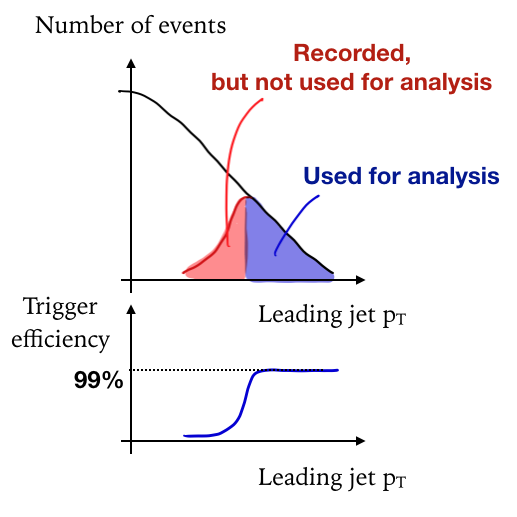
\includegraphics[width=0.5\textwidth]{figures/efficiencySketch}
\caption{\color{black}\label{fig:wastedRate} \small Sketch of how trigger inefficiencies caused by a mismatch between the HLT and offline jet energy scales causes events to be recorded but never used for analysis.} %Trigger operation page
\end{center}
%\vskip-5pt
\end{figure}

%maybe this is too big picture? but hey, a plot! 
The use of HLT objects for physics analysis provides further motivation to improve the trigger system and to optimize object reconstruction, benefitting the entire experiment.
Differences in the energy scale of HLT and offline objects also lead to inefficiencies in the trigger selection, as events that should pass the trigger are rejected due to miscalibration in the HLT. 
As an example, the minimum $p_{\rm{T}}$ threshold applied to jets used in physics analysis is set to be higher than the HLT threshold due to these differences, leading to a substantial waste in terms of events that are recorded but not used for analysis, as shown in Fig.~\ref{fig:wastedRate}. 
The application of TLA-motivated improved calibration constants at the HLT during e.g. LHC technical stops (allowing sufficient time for the reoptimisation of the trigger menu) can improve the fraction of useful data recorded and impact the overall ATLAS data-taking. 

\textbf{Analysis workflow for TLA and TLA+PEB}

In order to enable validation of the performance of TLA and TLA+PEB physics objects, it is necessary to retain an event format that includes both regular physics objects and objects presents in the reduced data formats, for a subset of the data.  

%edits by Teng Jian Khoo
TLA and TLA+PEB end-to-end analysis workflows enable a variety of physics analyses that are infeasible using conventional triggers due to high data taking rates. The TLA-only workflow has so far been running in the shadow of traditional workflow, both in terms of CPU and in terms of storage. In the future, the addition of more complex objects to reconstruct at the HLT as well as the addition of information in the reduced event data format will expand analysis prospects at a fraction of the cost of traditional workflows, but still not be completely cost-free. For this reason, the physics motivation and resource needs will need to be considered in the resource planning of the overall ATLAS physics program.

%Q for Lukas/Alison/Gordon: this section is pretty bare but I could add a diagram or write more, what do we want to do here? 

%Other things that could be added: 
% More of a resource discussion...
% Advantages of doing this beyond storage: code optimization, avoiding duplication, reduced waste of data (this is calibration and probably belongs to the analysis section?)
% Downsides: need more resources if everyone wants their own PEB so one needs to consider what gets saved carefully depending on the physics case
% More details on how one could do reconstruction in partial regions (= learn from trigger)

\subsection{Impact}

%How is the above mentioned R\&D expected to impact physics or costs to the experiment (not sure if this should be here or sprinkled through out this section).
%The activity's impact should be in terms of the "goals" set out in the introduction.

\section{Resource estimates}
%Davide, Armin, Giulio

\subsection{Summary of the parameters used for resources extrapolation}
A table with the parameters that are used for the resources extrapolation is provided. These parameters are in three categories,  (i) computing parameters such as CPU usage per event and event size, and (ii) computing model parameters such as number of replicas and number of (re)processings needed, (iii) physics parameters such LHC luminosity, trigger rate and number of events to be simulated 
The 
\subsection{The method used}
A short description of the python model used and how parameters dependencies can be studied independently. A derivative of the resources vs parameter should be  calculated, so the parameters with the largest impact on resources are listed

%\subsection{Possible scenarios}
%Different scenarios are identified. From a minimal %scenario where we do data reconstruction and little %simulation to the "ideal" scenario where we do all %simulation we need. The dependency on fast vs G4 %simulation is expected to be quite important 

\subsection{Projections for the Three Scenario}
Provide CPU, disk and tape needed projections in the Conservative, Baseline, and Aggressive scenarios. Provide resources extrapolations for 10\%/year and 20\%/year increases.

All the plots are ATLAS internal,  the parameters are still being discussed.    
Plots on the impact on physics performances should also be added, either here or in a different section





\begin{figure}[h]
    \centering
    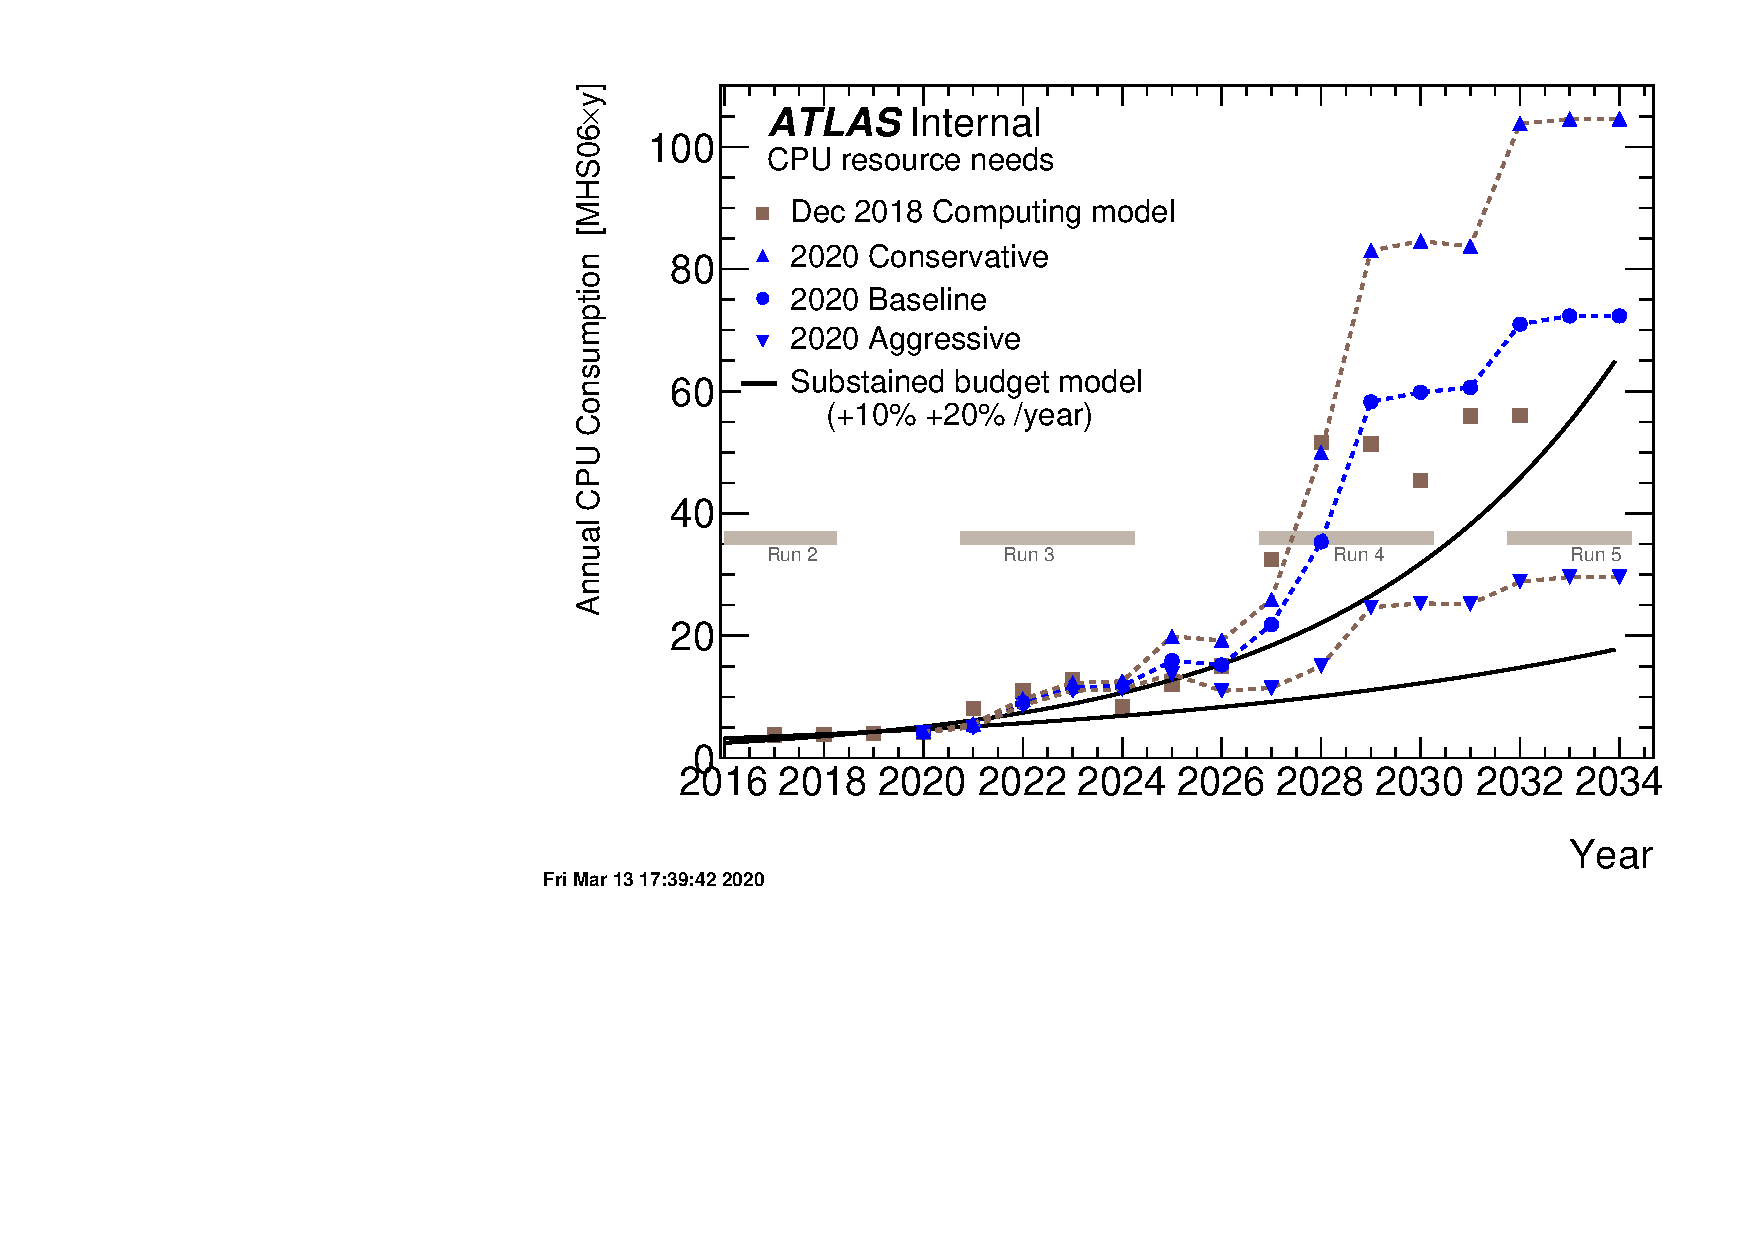
\includegraphics[width=0.80\textwidth]{figures/cpuHLLHC_comparison_2020_InputData_11March.pdf}
   \caption{ Estimated total CPU resources  needed  for the years 2020 to  2034.    }  
    \label{fig:cpu}
\end{figure}





\begin{figure}[h]
    \centering
    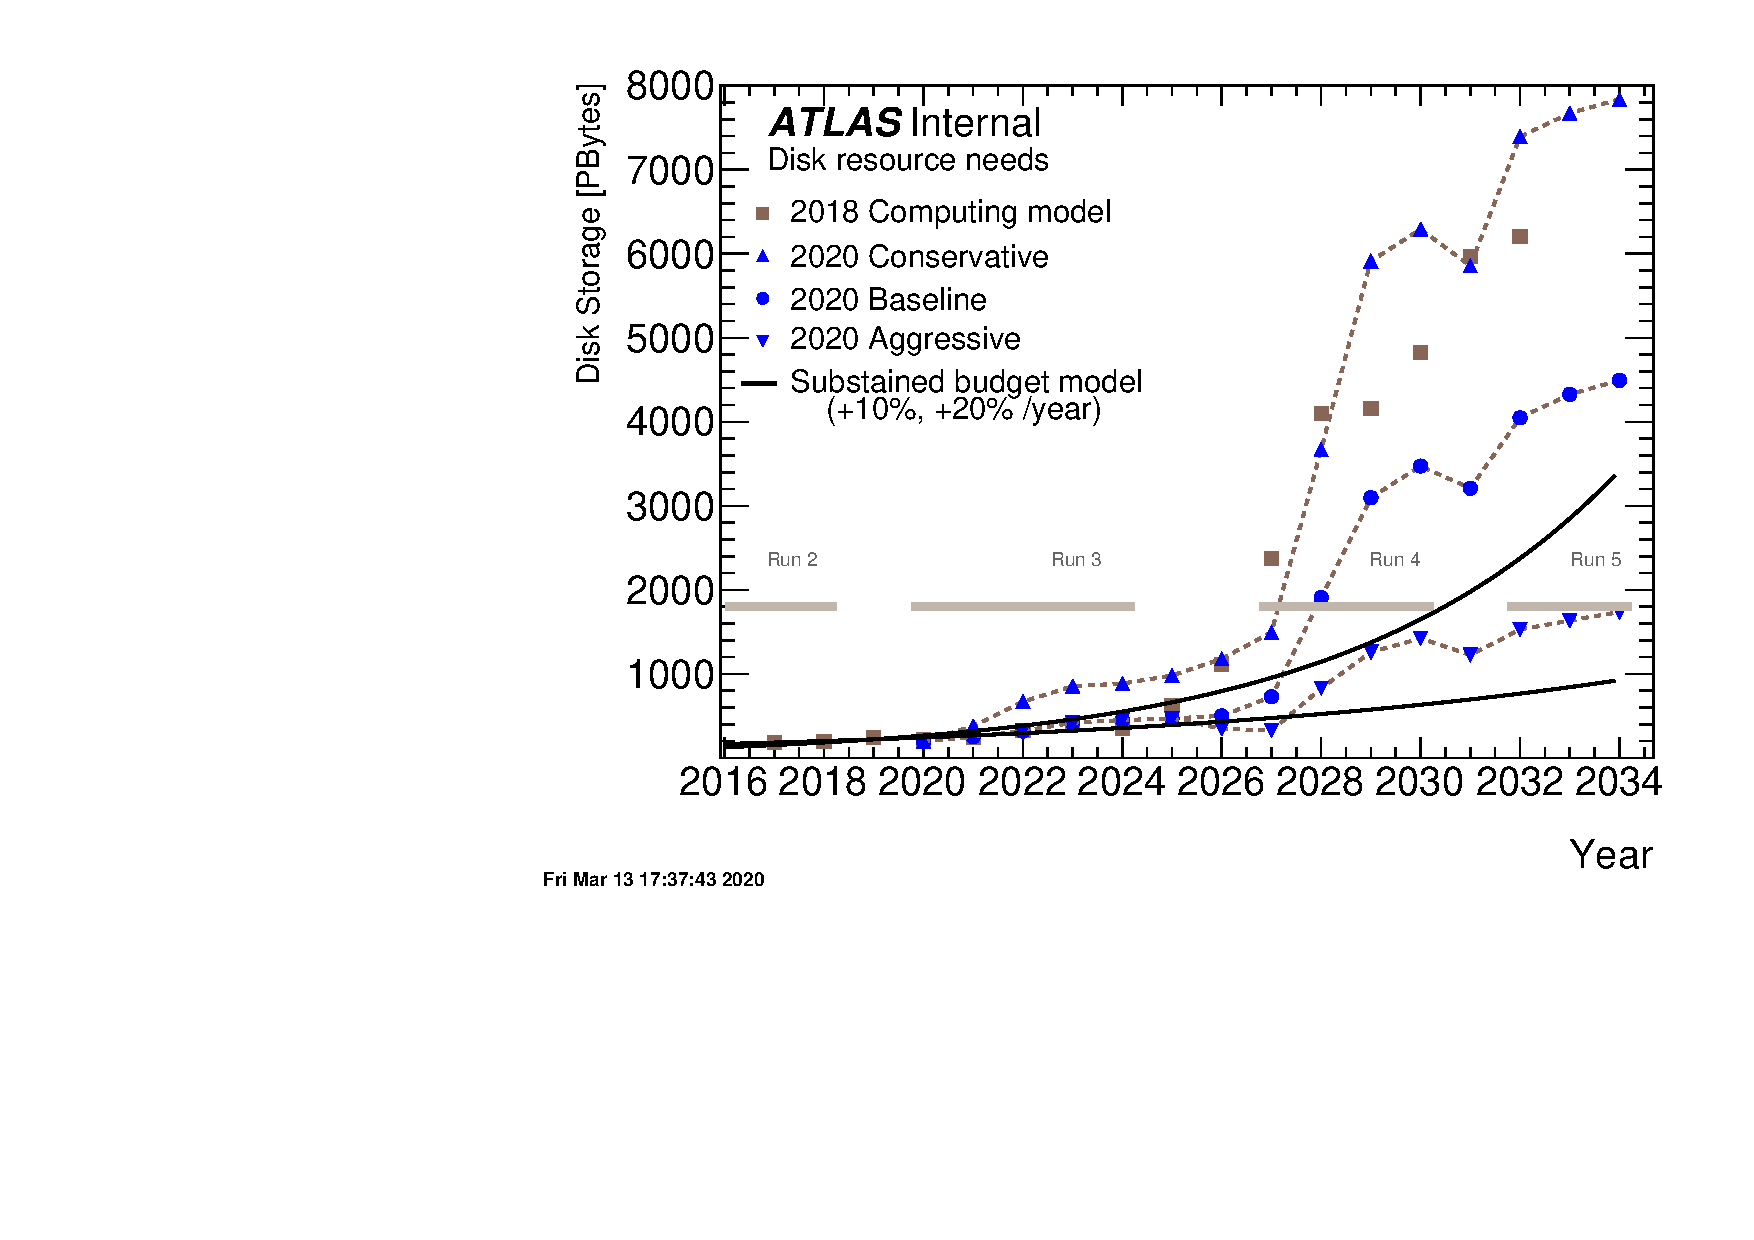
\includegraphics[width=0.80\textwidth]{figures/diskHLLHC_comparison_plot_2020_InputData_11March.pdf}
   \caption{ Estimated  total Disk resources  needed for the years 2020 to 2034.  }  
    \label{fig:disk}
\end{figure}




Here we update the plots that have been shown. We should have plots also for tape (or long-term storage) needs. 
Plots on the impact on physics performances should also be added, either here or in a different section

%\section{The role of Machine Learning}
% Dan, Amir, Lukas
%Machine learning will play an increasing role in LHC data analysis in the coming years. Applications for machine learning range from mature algorithms for particle reconstruction (cite b-tagging, tau-id, jet tagging, electron calibration) and event selection (cite overview, too many to count) to developing projects such as generative neural networks for simulation and interpolation over high-dimensional BSM model spaces. Given the wide range of potential applications, estimates of expected computing requirements come with a large error margin.

At the moment the computing demands for machine learning are relatively modest.... (Training is G/CPU intensive, inference is a single pass algorithm which is relatively fast) (ideally get some numbers on a typical training time)

(something about how the regular data structures we use in ML are conducive to vectorization / GPUs, thus might be cheaper than iterative algorithms. This might justify using a lot more GPU / ML in reconstruction)

As Machine Learning is a research field mainly driven by groups outside of particle physics, it is expected that the most performant frameworks for developing ML algorithms are developed in their respective communities. It is therefore prudent to maintain a clear boundary between training and inference frameworks. Only the latter needs to be requires integration into most HEP software and an emerging industry standard for sharing ML models is e.g. ONNX.



The basis of modern deep learning is the notion of numeric programs for which free parameters can be determined using gradient-based learning. Crucially, gradient of these programs can be efficiently computed through automatic differentiation techniques. While the future developments in ML are difficult to predict it is expected that the notion of \emph{differentiable programs} will remain foundational. In HEP, a number of projects have already begun exploiting autodifferentiatino (Pierini etc al for diffable likelihoods, pyhf, Tensorfloow fits in CMS) enabling a more direct integration of ML methoods with HEP through e.g. end-to-end learning.

The role of ML at the HL-LHC. This is where we try to form a more consistent picture of how all the other sections fit together.
\begin{itemize}
    \item applications
    \item computing overhead
    \begin{itemize}
        \item training
        \item inference
    \end{itemize}
    \item Industry tools and resources
    \item Hardware and GPUs
\end{itemize}

\section{Tier-0 and HLT farms, CERN infrastructure}
%Armin, Frank
\subsection{Trigger and DAQ}

The Phase-II upgrade of the ATLAS Trigger/DAQ (TDAQ) system and its Event Filter (EF) is described in detail in Ref.~\cite{ATLAS-TDR-29}. The EF system processes the events in almost real-time, takes the final trigger decision and assigns events to data streams. The EF farm will be built from commodity CPU servers with the optional addition of accelerators (GPU, FPGA) if they are found to be cost effective. The Dataflow system stores the accepted events in files and publishes them to the offline system. The Dataflow system is able to buffer events for up to 48 hours if needed.
During non-taking periods the EF farm acts as a standard Grid site and can be used to run e.g. simulation jobs ("Sim@P1").

Based on the current trigger menu draft (\cite{ATLAS-TDR-29} Table 6.4) an average EF output rate of 10~kHz at $\mathcal{L}=7.5\times10^{34}\,\mathrm{cm^{-2}s^{-1}}$, corresponding to approximately 200 inelastic proton-proton collisions per bunch crossing, is expected. This rate includes the main physics stream(s) but does not include detector calibration or Trigger-level Analysis (TLA) streams. TLA streams typically have a very high rate but with very small event sizes of the order of 10~kB. Based on data from Run-2, those additional streams contribute about 20\% of the total bandwidth and storage at the Tier-0. 

The estimated event size for each detector system at the ultimate Phase-II luminosity is listed in Table~\ref{tab:event_size} resulting in a total average event size of 3.6~MB.
This is a significant reduction compared to the 5.2~MB listed in the TDAQ TDR (\cite{ATLAS-TDR-29}, Table 3.5) due to the reduction in the Pixel event size in the latest iteration of the readout chip~\cite{ATL-ITK-INT-2019-001}. The event size of the new High-Granularity Timing Detector (HGTD) has been taken from Figure~4.26 in Ref.~\cite{ATLAS-HGTD-TP}.
Allowing additional bandwidth for calibration and TLA streams, the total bandwidth to Tier-0 is approximately 45~GB/s.

\begin{table}[htb!]
    \centering
    \begin{tabular}{|c||c|c|c|c|c|c|c||c|} \hline
         Detector & Pixel & Strip & HGTD  & LAr   & Tile  & Muon  & TDAQ  & Total \\ \hline
         MB/event & 0.6   & 0.5   & 0.2   & 0.7   & 0.2   & 0.8   & 0.6   & 3.6 \\ \hline
    \end{tabular}
    \caption{Expected average event size at $\langle\mu\rangle$=200. Forward detectors are not listed since the associated event size is negligible.}
    \label{tab:event_size}
\end{table}


\subsection{Tier-0}

It is clear that the Tier-0 will have to provide sufficient network bandwidth and storage capacity (both disk and tape) to enable basic RAW data recording, archival, and export to Tier-1/2 centres. Section~\ref{sec:tier0_network} presents estimates on the Tier-0 network capacity for Run 4.

Performing the processing of data at Tier-0 in Run 4, in the way it was done in Runs 1 and 2, and will be done in Run 3, will require a substantial upgrade of the Tier-0, in the most optimistic scenarios by factors of 4--6. Section~\ref{sec:tier0_capacity} gives estimates on the required CPU capacity, depending on the reconstruction timing estimates of Section~\ref{sec:reco}. How much of such a Tier-0 upgrade will be affordable, is not yet known. Depending on the available processing capacity at Tier-0, various processing scenarios are discussed in Section~\ref{sec:tier0_workflows}.

\subsubsection{Tier-0 Network Traffic}
\label{sec:tier0_network}

Assumptions: 

\begin{itemize}
  \item RAW data recording: 10~kHz physics rate, ca.\ 3.6~MB full physics event size (estimate for $\langle\mu\rangle$=200, cf.\ Table~\ref{tab:event_size} above), 20\% of bandwidth occupied by non-physics streams (calibration, TLA, etc.); 
  \item 70\% LHC time in stable beams;
  \item RAW data backed up to tape and exported to Tier-1s as fast as possible (``live'');
  \item Tier-0 processing spread over fill and inter-fill periods ($\Rightarrow$ scale factor 0.7 applied on data rates);
  \item Reconstruction outputs: AOD of 350~kB/event, total data volume of other products (DRAW, performance DESD, DAOD, etc.) not more than that of AOD; 
  \item Merging of reconstruction outputs in a separate, subsequent step;
\end{itemize}

Table~\ref{tab:tier0_rates} shows the estimates on the required Tier-0 network traffic and bandwidth.

\begin{table}[htb!]
\begin{center}
  \begin{tabular}{|c|c|c|c|c|}
    \hline
    {\bf Activity}                 & {\bf EOS Read}    & {\bf EOS Write}   & {\bf CTA Read} & {\bf CTA Write}      \\\hline\hline
    DAQ: SFO $\rightarrow$ EOS     & --                & 43~GB/s           & --             & --                   \\\hline
    Tier-0: Reconstruction         & 25~GB/s           & \phantom{4}5~GB/s & --             & --                   \\\hline
    Tier-0: Merging                & \phantom{4}5~GB/s & \phantom{4}5~GB/s & --             & --                   \\\hline
    DDM: Export to Tier-1s         & 48~GB/s           & --                & --             & --                   \\\hline
    DDM: EOS $\rightarrow$ CTA/EOS & 48~GB/s           & --                & --             & 48~GB/s              \\\hline
    CTA: Tape Backup               & --                & --                & 48~GB/s        & 48~GB/s              \\\hline\hline
    {\bf Total}                    & {\bf 126~GB/s}    & {\bf 53~GB/s}     & {\bf 48~GB/s}  & {\bf (48 + 48)~GB/s} \\\hline
  \end{tabular}
\end{center} 
\caption{Estimated Tier-0 network traffic for Run~4.}
\label{tab:tier0_rates}
\end{table}


The figures do not contain contingencies. To be on the very safe side, one might want to add extra capacity of 30--50\%. On the other hand, a fraction of 70\% in stable beams is a very optimistic assumption that already leaves some headroom.

\subsubsection{Tier-0 CPU Capacity}
\label{sec:tier0_capacity}

Assumptions: 

\begin{itemize}
  \item 10~kHz physics rate;
  \item 80\% of CPU used for physics processing, 20\% for everything else (calibration/alignment, DQM, merging, etc.);
  \item 70\% LHC time in stable beams ($\Rightarrow$ 7~kHz effective reconstruction rate required);
  \item Reconstruction timing estimates according to Section~\ref{sec:reco}, Table~\ref{tab:Phase2CPU}; 
\item Tier-0 cluster capacity at the end of Run~2 (2018): 430~kHS06.
\end{itemize}

Table~\ref{tab:tier0_cpu} shows the estimates on the required Tier-0 CPU capacity.

\begin{table}[htb!]
\begin{center}
  \begin{tabular}{|c|c|c|c|c|}
    \hline
    {\bf Pile-up}             & {\bf Reco.\ Time/Event} & {\bf Required CPU Capacity} & {\bf CPU Capacity wrt.\ Run~2} \\\hline\hline
    $\langle\mu\rangle =$~140 & 402 (215)~HS06$\cdot$s  & 3500 (1900)~kHS06           & \phantom{1}8.2 (4.4)           \\\hline
    $\langle\mu\rangle =$~200 & 584 (295)~HS06$\cdot$s  & 5100 (2600)~kHS06           & 11.9 (6.0)                     \\\hline
  \end{tabular}
\end{center} 
\caption{Estimated Tier-0 CPU capacity for Run~4, for two scenarios: one based on Run-2 reconstruction, the other (in parentheses) on the target performance after a successfully carried out software upgrade programme.}
\label{tab:tier0_cpu}
\end{table}


\subsubsection{Considerations on Tier-0 Workflows in Run~4}
\label{sec:tier0_workflows}

Prompt processing at Tier-0 for calibration, alignment, beam-spot determination, data-quality montitoring (DQM), etc. will always stay one of the Tier-0 proper responsibilities. This kind of processing is time critical, it has to be accomplished within a time window of 48 hours (the so-called ``calibration loop''), and requires fast feedback and turnaround. It may also rely heavily on the local infrastructure, such as live DCS information from local conditions databases. Therefore this can only be done at Tier-0, the Grid is not suitable. 

In Run 2, O(10\%) of CPU resources were used for calibration- and alignment-related processing. One may expect that the total capacity needed to perform all the calibration processing will stay about the same. In any case it will not have to scale up 1:1 proportionally to the physics rate.   

In Run 3, it is foreseen that the Tier-0 will have sufficient capacity to perform all the bulk processing ({\it physics\_Main} stream), like in previous runs. Bulk processing is launched after the 48-hours' calibration loop. So far it has been a strong requirement (or preference) by the Data Preparation and Physics communities to do bulk processing in this way. The advantage is the fast availability of validated, uniform outputs which are directly useable for physics production. Accompanying DQM and other, e.g., CP-related, processing which relies on the full available statistics and often makes use of the local CERN infrastructure can be performed promptly as well. For instance, DQM results are used for run-by-run sign-off and the compilation of Good Run Lists. 

Already since Run 2, the Tier-0 batch farm has been configured in a way that its CPU resources can be shared between Tier-0 and Grid processing. In periods of data taking and processing, Tier-0 runs with priority, else the Grid takes over. This makes sure that the available, sizeable capacity is always efficiently used. Therefore, if for Run 4 and beyond the Tier-0 capacity were extended according to Table~\ref{tab:tier0_cpu}, such that all prompt and bulk processing could be performed there, there would be no risk of resources running idle or being wasted in periods of no data taking -- they would just be used by the Grid. 
 
From today's perspective, based on existing workflows, at least some amount of statistically representative data (comparable to today's {\it physics\_Main}) would need to be reconstructed promptly for DQ assessment, CP studies, monitoring, etc. 

If resources at Tier-0 were not sufficient to do all the prompt processing, one could envisage to split off 10--20\% of data to process at Tier-0 for DQ (something like a {\it ``physics\_Monitoring''} stream) and do the rest across the Grid. One could even consider an LHCb-like model in which RAW data for selected streams are deleted after prompt reconstruction, in order to save on storage. However, the 10--20\% of extra bandwidth and storage, even for transient {\it ``physics\_Monitoring''} data, might be an issue that needed to be addressed.

In case resources at Tier-0 were not sufficient to do all the prompt processing, ``spill-over'' to the Grid would be an option that could be explored.

Spill-over was demonstrated to work, functionally (on {\it physics\_Main} for some runs, for validation purposes), and in routine operation in 2018 (on {\it physics\_BphysLS} stream, ca.\ 100~Hz, ca.\ 10\% of {\it physics\_Main}). Tasks were defined at Tier-0 and injected through a python API into the Grid Production System. Reconstruction and merging were run on the Grid, outputs (AOD, HIST) had to be shipped back to CERN for further special (DQM, CP) processing at Tier-0 that could not be done on the Grid. Back-feeding Grid outputs into Tier-0 was tedious, as Tier-0 and Grid Production Systems are separate entities. 

Tier-0 looks to be the natural place to manage, define, and orchestrate the spill-over (as it knows about data availability, readiness of calibrations and software; it is the hub between T/DAQ, calibration/alignment groups, Data Preparation, and distributed computing communities; etc.). If resources at Tier-0 were so short, however, that a dominant fraction of bulk processing would need to be performed on the Grid, it would make more sense to move the responsibility for organising and executing bulk processing to the Reprocessing and Grid Production domains altogether. 

In all those scenarios, more development towards an easier interaction between the Tier-0 and Grid Production Systems, and a better integration of the respective monitoring tools and interfaces, would be desirable, in order to fully and efficiently exploit the potential of the spill-over. This could be addressed and exercised in Run 3 already, however. 


\section{Evolution of distributed computing}
%Oxana, Rod, Kaushik + DDM group
% Guidance: maximum 3 pages for this section. Since we have 6-7 sub-sections, each should be 1/2 page maximum.

We anticipate that distributed sites will continue to provide the bulk of resources used for data processing, simulations and analysis in the HL-LHC era. This infrastructure is expected to be provided via WLCG mechanisms based on bilateral agreements (MoU) between WLCG and contributing funding agencies that cover the entire duration of the LHC program, including HL-LHC. ATLAS has a sophisticated distributed computing system (ADC) that optimally makes available hundreds of clusters and associated storage at distributed WLCG sites. ADC provides a fully integrated system for all workflows and for all users. The automated tools developed by ADC include ProdSys, PanDA, Rucio, SSB, HammerCloud, and others. These tools will continue to be upgraded and evolve as needed. Many of the upgrade plans require tighter future integration among tools to improve efficiency in the more complex environment of the HL-LHC. Below we provide a few examples of long range R\&D plans which are needed to transition to the new challenges at the HL-LHC. The metrics used to evaluate progress with the R\&D projects will include: scalability for HL-LHC, improved efficiency in resource usage (CPU, storage and network), and improved operational efficiency. We anticipate all the new R\&D projects described here will require additional effort or redirection of effort.

\subsection{Evolution of WLCG}
\label{sec:wlcg}

WLCG strives to accommodate many scientific endeavours in future, and already now DUNE~\cite{DUNE2018} and Belle-II~\cite{Belle-II} have joined the infrastructure. More projects are expected to join soon, most notably, those that take part in the European ESCAPE~\cite{EU-ESCAPE} cluster of ESFRI activities. The overarching challenge for all these projects is distributed data handling, therefore WLCG focuses on R\&D in the areas of Data Organisation, Management and Access (DOMA), which is expected to have impact in terms of the data infrastructure and services. In particular, the Data Lake approach (see Section~\ref{sec:lakes}), under development and evaluation by current R\&D projects (DOMA, ESCAPE, IRIS-HEP, and others), will have implications on data placement, delivery and caching, which will need to be properly accommodated by ATLAS tools and services. Specifically, multi-level caching via Xcache, third-party transfer implementation without GridFTP, token-based authentication and quality of service criteria will have to be implemented in ATLAS distributed computing tools. 

Earlier (in Figure~\ref{fig:2018Res}) we showed the resource challenges facing the HL-LHC. Many R\&D activities have already started to address the CPU challenge -- we expect that the CPU deficit will be substantially reduced through these efforts described in other sections. However, the storage and network challenges are formidable, which will be partly addressed through the WLCG DOMA project. Later in this section we describe a few additional R\&D projects to manage the storage shortfall, like Data Carousel and iDDS, which are specific to ATLAS.

%how do we make it quantitative?

\subsection{PanDA and ProdSys}

PanDA is the ATLAS workload management system used to execute all scientific workflows for all users on widely distributed heterogeneous resources. It is tightly integrated with the ATLAS distributed data management system, Rucio. For the HL-LHC, the PanDA development team has started multiple R\&D efforts. The Data Carousel project, the ProdSys system, HPC and cloud orchestration, and the intelligent Data Delivery System are prominent examples described separately. In addition, the PanDA team is working on global shares and unified queues, edge services through Harvester, MPI services, event service, SciTokens authentication, active network management, operational intelligence, anomaly detection, and machine learning techniques. We anticipate that one to two FTE effort will be needed for these R\&D topics for the next three years. The overall goal is to meet the HL-LHC scale and resource capacity challenges without sacrificing the flexible ADC system.

ProdSys is the primary interface between users and PanDA, providing a task management interface. New workflows are regularly developed in ProdSys. Monitoring systems are evolved to meet new requirements. The most disruptive challenge facing ProdSys is the growing importance of machine learning techniques, especially for distributed training. New schemas are being developed for non-traditional HEP use cases that are not collision event based. As new analysis models emerge for HL-LHC, we expect major additions to ProdSys capabilities. R\&D efforts in ProdSys for the HL-LHC will be primarily focused on supporting non-traditional workflows. We estimate this effort to require half FTE over three years.

\subsection{Rucio}

Rucio is an open-source software framework that provides scientific
collaborations with the functionality to organize, manage, monitor, and
access their distributed data at scale. The system manages more than 500
petabytes spread on 130 data centres with 600 storage locations, with
daily data access of over 12PB, as well as over 2PB of data transfers,
deletion, and recovery. The success of Rucio in the ATLAS experiment has
led to it being adopted as the data management system by the CMS,
XENON-1T, and AMS experiment and it is under evaluation by several other
established and upcoming experiments such as Belle 2, DUNE, LIGO/VIRGO,
and SKA.

Future developments, specifically aimed at the HL-LHC era, aim to
further improve the scalability of the system, to ensure that the system
scales to the requirements of HL-LHC data rates. These developments are
already starting now and especially target the improvement of the
deletion and transfer evaluation components of the system. Further
developments are planned to evolve the metadata component to support
future workflows as well as to introduce the functionality of storage
Quality of Service (QoS) to the system. Although Rucio already supports
numerous database back-ends, such as Oracle, MySQL, and PostgreSQL,
special emphasis is being made to ensure that the database interactions
scale for Non-Oracle databases. Additionally, as more experiments and
communities at similar data rates as the HL-LHC will come online in the
next years, another development will be orchestration of dataflows
across multi-experiment Rucio installations, as well as direct
integration with the network layer for dynamic provisioning of bandwidth.

% Can Rucio team provide estimate of how much additional effort is needed for R&D?

\subsection{Data Carousel and iDDS}
The cost of disk storage will be prohibitive for our current workflow patterns at HL-LHC volumes. We must therefore make better use of cheaper media with lower QoS - today this means magnetic tape, but the method does not exclude others, for example spun-down hard disk.
The Data Carousel orchestrates data processing across workload
management, data management, and storage services with the bulk data
resident on offline storage. The processing is executed by staging and
promptly processing a sliding window of inputs from faster buffer storage,
such that only a small percentage of input data are available at any time. With this project we aim to demonstrate that this is the natural way to
dramatically reduce our storage cost. The first phase of the project was
started in the Autumn of 2018 and was related to I/O tests of the sites archiving
systems. Phase II requires a tight integration of the workload and data management systems and will be used already in Run3 for processing RAW data. At HL-LHC we will need to go further and store reconstructed data principally on tape, to be processed using the Data Carousel. This will require further developments such as 
file level staging-job orchestration through intelligent Data Delivery Service (iDDS). The iDDS system in PanDA is being developed to provide streaming services for data delivery for a wide range of workflows. Data Carousel is an important and first proof of concept demonstration of iDDS for ATLAS.

%\subsection{Streaming Data Services}
%In order to support new analysis methods \cite{streaming} we will need to produce custom data formats in quasi-realtime and stream to user analysis facilities. ServiceX will produce data in a columnar format suitable for highly parallel processing. iDDS would enable a user feedback loop into multi-step analysis chain.
% not sure I understand this, but both are referenced from the analysis section

%\subsection{Machine Intelligence for Workflow Management}
%KD


\subsection{Infrastructure}

\subsubsection{Facilities and operations}

%IMPORTANT: stress the need for "own" custom facilities, as opposed to generic HPC ones. Do we have to speculate on evolution of facilities? Containerized Data Centres? Microservices? DevOps?
%Tier 1 vs Tier 2 difference is gone (except for tape and 2nd copy of data)
%evolve towards facilities based on capability rather than Tier label

While the rigid hierarchical distinction between Tier 1 and Tier 2 sites already disappeared in ATLAS during Runs 1 and 2, these sites will continue to be the backbone of the computing infrastructure for ATLAS at the HL-LHC. Tier 1 sites are expected to continue providing custodial service for primary data through tape storage. A more flexible classification of sites based on capabilities is emerging. Sites will be classified based on infrastructure and workload capabilities irrespective of their Tier label. HPC, Cloud and other opportunistic resources are expected to extend the capabilities of ATLAS managed Tier 1 and Tier 2 sites, but not replace their custodial roles or provide the wide array of time critical processing and storage services.

\subsubsection{Analysis Facilities}
During Runs 1 and 2, WLCG Tier 1 and 2 sites provided distributed processing capability for ATLAS analysis users, at the scale of a million analysis jobs executed per day. However, these facilities are not well suited for the final interactive stages of user analysis, for example visualizations, plot generation, re-weighting, systematic studies, limit testing, etc. Local sites (often called Tier 3 sites), funded and managed outside the WLCG framework, often provided the necessary resources for end-user analysis. Many of these sites are connected through ADC tools like PanDA and Rucio. The future of these analysis facilities depends on the success of new analysis tools and analysis models. R\&D work is needed to determine the size, scale and cost of analysis facilities. Metrics of reduced cost, increased efficiency and scalability need to be demonstrated. This R\&D work is dependent on the analysis tools R\&D described earlier in the document, and will require additional effort of a few FTE to evolve the future analysis facilities.


\subsubsection{Data Lakes}
\label{sec:lakes}
A possible future direction for WLCG storage is to extend the concentration of disk resources at fewer and larger, possibly federated, sites. Smaller cache-like storage would serve the more widely 
distributed computing resources. The reasoning is that the provisioning and operation of robust storage requires significantly more manpower, than needed for a compute cluster with a cache of secondary replicas. In principle, distributed operations are simplified in this scenario, although separation of storage and computing raised their own reliability and operational challenges in the past. Results from a WLCG survey suggest the manpower requirement is perhaps not a driving factor for the typical Tier2. Also local and regional funding tends to work against concentration of resources. Nevertheless, some sites or funding agencies have already chosen to connect computing facilities to remote storage through cache layer. We need to prepare for a significant fraction of remote accesses.

\subsubsection{Network}
\label{sec:network} 
The exponential growth of essentially free research network bandwidth has thus far enabled an abstraction of the ATLAS data transfer activities from the underlying network. The major developments likely to affect ATLAS are packet marking, new cost models and programmable WAN links.  

Packets traveling on dedicated WLCG sections of the network will be marked by the application, in order to attribute the activity to a particular Virtual Organization (VO). This capability is especially important because it is not always clear what the impact to wide-area networking is when making changes to our complex, global infrastructure. Being able to identify owners and types of traffic flows anywhere in the network makes it possible to identify the root cause for significant changes in network traffic.  Another consideration is that the cost for a particular bandwidth, for example transatlantic, may become more direct, rather than hidden in general research network budgets. In addition, usage of commercial cloud storage egress incurs very clear costs for the experiment.  Programmable WAN links offer the potential to be able to boost bandwidth between sites on demand.

Rucio has a matrix of connectivity and bandwidth between sites, with information taken from the File Transfer Service (FTS) and manual input. This will be augmented with information about cost and potential programmable links. PanDA can use this to influence job placement, but will need improvements to optimize for speed or cost.

Much of this work is being discussed in twice yearly LHCONE/LHCOPN meetings and has been reported on by the HEPiX Network Function Virtualization working group in their phase I report\cite{hepix_nfv_working_group_2019_3565563}.  

It is important to note that ATLAS will need to work more closely with both the national research and education networks and the various networking research efforts to effectively prepare for the HL-LHC era. In early 2020 there are efforts underway to create a networking technical working group to discuss, document and prototype capabilities identified as being important for the LHC experiments.  ATLAS also needs to be ready to take advantage of international scale network testbeds capable of providing a geographical footprint, advanced services and capacities relevant for the HL-LHC.  Testbeds like that will be critical for testing network capabilities and services to evaluate their impact for ATLAS in the context of HL-LHC. 

%Need to cut down HPC section below to fit 1/3rd to 1/2 page. Seems cut already.

\subsubsection{Non-dedicated High Performance Computing resources}
\label{sec:hpc}

Due to the large amount of data used by ATLAS, currently about half an Exabyte for all data products and growing, and custom developed software applications specific to ATLAS, it is considered optimal for ATLAS to use dedicated resources at Tier 1 and Tier 2 sites, starting with specially configured networks (Sec.~\ref{sec:network}), storage facilities (Sec.~\ref{sec:lakes}) and computing resources. These sites are mostly large clusters similar to those at CERN. The vast majority of resources pledged by contributing countries and those used for Runs 1 and 2 at the LHC, are thus hardware built for ATLAS and other LHC experiments. Without these dedicated resources, some computing workflows will need to be rationed, thereby reducing the scope of physics results produced by ATLAS. It is anticipated that the current resource deployment will continue in the future: most national particle physics communities will retain the ability to build and maintain dedicated IT infrastructures for ATLAS needs.

Historically, some significant resources were pledged to ATLAS through allocation or dedicated partitions at generic public High-Performance Computing facilities. One notable example is the NDGF Tier1~\cite{ndgf} where all computational power is provided via national research data centers shared with other scientists. It is anticipated that in future more resource providers will use this model, and a larger part of the pledged resources will come through non-dedicated shared facilities. While they will still be a part of the WLCG infrastructure, ATLAS will have to cope with the necessity to adapt to such resources in terms of e.g. processor architectures, operating systems, file systems, quotas etc.

% Bibliography is needed for Leadership machines and backfill success stories
At the same time, very large HPC facilities, for example the Leadership Class Facilities~\cite{leadership} funded by the U.S. Department of Energy, are known to have large idling capacity due to the nature of their main workloads. Such facilities are willing to accept serial payloads from ATLAS as a back-fill~\cite{backfill}. With an increased investment in Europe and worldwide into exascale computing it is safe to assume that more such opportunities will appear in future, and a significant computing capacity will become available opportunistically, i.e., outside of the service levels as defined in the WLCG MoU~\cite{wlcg-mou} and not subject to WLCG policies and operational procedures in general. In this case ATLAS will have to cope not only with local architecture peculiarities and policies, but also with the fact that such facilities are not a part of the WLCG operations. This will limit the workloads that we can run, and part of the preparations for HL-LHC will be R\&D to run more challenging workloads, such as data-intensive or those requiring extensive database access at HPC sites. This can only work if HEP requirements are taken into account in both the design and policies of the HPC facilities. We estimate one FTE additional effort for HPC R\&D.


%\begin{figure}[ht!]
%\caption{Evolution of the share of accelerators and co-processors in Top500 HPC systems %(source: top500.com). A trend towards an increasing share of such can be seen.
%\label{fig:top500-gpu}}
%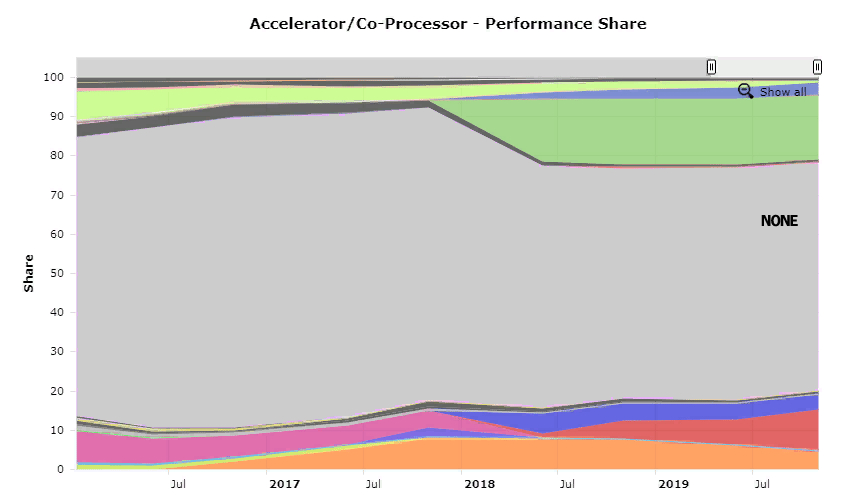
\includegraphics[width=12cm]{figures/Top500-coprocessors.png}
%\end{figure}

%Challenges:
%\begin{itemize}
%    \item Heterogeneous architectures are likely to become dominant, implying that less capacity will be available through conventional CPUs. % see Fig.~\ref{fig:top500-gpu}.
%    \item Opportunistic resources have no formal Service Level Agreements consistent with the rest of the infrastructure.
%    \item Local to HPC policies may be inconsistent with ATLAS ones, such as e.g. limited access to users outside the host country.
%\end{itemize}

%\section{Evolution of database}
% Elizabeth, Nurcan, Dario
%the wonderful evolution of databases . 

%\section{Physics impact of the various scenarios}
% This may or may not be needed, as it could be embedded in the various sections. 
%Davide and Paolo to propose scenarios
%Simone, Sara, Christian

\section{Effort estimates and high level milestones}
% Ale and James
effort and milestones

\bibliography{bib/ATLAS.bib,bib/misc.bib,bib/visualization.bib,bib/physics.bib}
\bibliographystyle{plain}

\end{document}
